\documentclass[twoside]{scrartcl}
%\documentclass[numbers=noenddot]{scrbook}	%ohne numbers=noenddot sähen die Section so aus: 3.3. Module
\usepackage[utf8x]{inputenc}
\usepackage[english,german]{babel}
%\usepackage[a4paper]{geometry}
\usepackage[a5paper]{geometry}
\usepackage{amsmath,amssymb,amsthm,amstext}		%AMS Pakete; \text{}
\usepackage{gensymb}					%definiert \ohm
\usepackage[pdftex]{graphicx}			%Paket für Bilddateien
\usepackage[usenames,dvipsnames]{xcolor}						%Paket für Farben
\usepackage{pdflscape}
\usepackage{hhline}
%\input{GraphicsMacros}
%\usepackage{fancybox}					%Boxen, genutzt für die Erklärungsbox(en)
\usepackage{fancyvrb}					%Boxen mit Verbatim-Inhalt
\usepackage[Sonny]{fncychap}			%anders formatierte Kapitelüberschriften, mögliche Parameterwerte: Sonny, Lenny, Glenn, Conny, Rejne, Bjarne

%folgende Pakete sind aus 'Der \LaTeX Begleiter' von Michel Goossens, Frank Mittelbach, Alexander Samarin entnommen
%\usepackage[german]{varioref}			%\vref{schlüssel}, \vpageref{schlüssel}
%\usepackage{doublespacing}				%\begin{spacing}{1.5} ... \end{spacing}	%gibt es nicht :(
%\usepackage{picinpar}					%\begin{figwindow}[anzahl zeilen vor dem fenster, position lcr, {\fbox{\includegraphic{}}, Bildunterschrift] \end[figwindow}
%\usepackage{program}					%\begin{programbox} programmcode... \end{programbox}
\usepackage{tabularx}					%wie tabular ABER bestimmt die Spaltenbreiten selbst! \begin{tabularx}{tabellenbreite z.B. \linewidth}{l|l|l|..} \end{tabularx} mehr aus Seite 116
\usepackage{colortbl}					%farbige Zellen mit \cellcolor{gray}
\usepackage{multirow}
\usepackage{multicol}
%\usepackage{colortbl}					%definiert \cellcolor{farbe}
%\usepackage{delarray}					%sinnvoll bei Matrizen oder abschnittsweise definierten Funktionen, mehr auf Seite 119
%\usepackage{floatflt}					%\begin{floatingfigure}{breite} .. \caption{} \label{} \end{floatingfigure}
\usepackage{wrapfig}					%ähnlich floatfig, aber keine automatische Positionierung der Abbildungen; siehe Seite 155
%\usepackage{float}					%
\usepackage{subcaption}
\usepackage{rotating}

%\usepackage{listings}					%zum Listen von Code
\usepackage{capt-of}

\usepackage{wallpaper}					%Hintergrundbild

\usepackage{tikz}						%"Malprogramm"
%\usetikzlibrary{decorations}
%\usetikzlibrary{arrows}
%\usetikzlibrary{calc}
%\usetikzlibrary{shadows}
%\usetikzlibrary{automata}
%\usetikzlibrary{matrix}
%\usetikzlibrary{trees}
%\usetikzlibrary{positioning}
%\usetikzlibrary{patterns}
%\usetikzlibrary{shapes}
%\usetikzlibrary{shadows.blur}
%\usetikzlibrary{shapes.symbols}
%\usetikzlibrary{circuits}
%\usetikzlibrary{snakes}	%mittlerweile in decorations enthalten
%\usepackage{pgfplots}
%\pgfplotsset{compat=1.3}
%\usepackage{pgfplotstable}
%\usepackage[siunitx]{circuitikz}
%\usepackage{tikz-timing}
%\usepackage{tikz-3dplot}

\usepackage{xifthen}

\usepackage[normalem]{ulem}

%\usepackage{abstract}					%funktioniert nur in der article oder report Umgebung

%\usepackage{mathptmx}					%Times New Roman				Normaltext & Formeln
%\usepackage{mathpazo}					%Palatino						Normaltext & Formeln
%\usepackage{courier}					%Courier						Text in Schreibmaschinenschrift
%\usepackage[scaled]{helvet}			%Helvetica 						Serifenloser Text
%\usepackage{bookman}					%Bookman 						Normaltext
%\usepackage{newcent}					%New Century Schoolbook 		Normaltext 
%\usepackage{avant}						%Avant Garde					serifenlosen Text
%\usepackage{charter}					%Charter						Normaltext
%\usepackage{chancery}					%Zapf Chancery					Normaltext
%\usepackage{palatino}
%\usepackage{mathpalo}
%\usepackage{chancery}
%\usepackage{times}
%\usepackage{eucal}						%calligraphic
%\usepackage{pifont}					%ZapfDingbats font \ding{number}
\usepackage{eurosym}
\usepackage{wasysym}					%Sternzeichen und anderes (\male, \female, \lightning, ...)

\usepackage[colorlinks]{hyperref}
\usepackage[figure,table]{hypcap} 		% Correct a problem with hyperref
\hypersetup{
	bookmarksnumbered,
	pdfstartview={FitH},
	citecolor={black},
	linkcolor={black},
	urlcolor={MidnightBlue},
	pdfpagemode={UseOutlines},
	pdftitle={Thinking Big},
	pdfauthor={Thorsten Spätling}
	pdfsubject={}
}
%\usepackage[
%%nonumberlist,	%keine Seitenzahlen anzeigen
%acronym,		%ein Abkürzungsverzeichnis erstellen
%toc,			%Einträge im Inhaltsverzeichnis
%section]		%im Inhaltsverzeichnis auf section-Ebene erscheinen
%{glossaries}			%gefunden auf http://ewus.de/tipp-1029.html

%\usepackage{attachfile}
%\attachfilesetup{color=.7 .7 1,icon=Paperclip}

\newcommand{\FOREIGN}[1]{\emph{#1}}
\newcommand{\TOWN}[1]{\textsf{#1}}
\newcommand{\TODO}[1]{\texttt{#1}}


\usepackage{makeidx}
%makeindex main.idx ausführen, danach kompilieren und der Index stimmt.

\usepackage{caption}
%\renewcommand{\figurename}{Abb.}
%\renewcommand{\tablename}{Tab.}
%\addto\captionsgerman{\renewcommand{\figurename}{Abb.}}
%\addto\captionsgerman{\renewcommand{\tablename}{Tab.}}
%\addto\captionsgerman{\renewcommand{\listingname}{Codebeispiel}}
%\addto\captionsngerman{
%\renewcommand{\figurename}{Abb.}
%\renewcommand{\tablename}{Tab.}
%}

\usepackage{scrwfile}	%normalerweise können nur 18 Dateien gleichzeitig geändert werden, damit soll dieses Handicap umgangen werden.

%\usepackage[euler]{textgreek}
\usepackage{textcomp}			%pfeile

%\usepackage{babelbib}	%deutsche Literaturverzeichniseinträge
\usepackage[fixlanguage]{babelbib}
\selectbiblanguage{german}

\usepackage{footnote}	%für Fußnoten in Tabellen

%\usepackage[titletoc]{appendix}
%\renewcommand{\appendixname}{Anhang}

\title{Thinking Big}
\author{Thorsten Spätling\\
{thorsten@ts-soft.info}}

%%%%%%%%%%%%%%%%%%%%%%%%%%%%%%%%%%%%%%%%%%%%%%%%%%%%%%%%%%%%%%%%%%%%%%%%%%%%%%%%
%%% Abgabedatum %%%
%%%%%%%%%%%%%%%%%%%%%%%%%%%%%%%%%%%%%%%%%%%%%%%%%%%%%%%%%%%%%%%%%%%%%%%%%%%%%%%%
%\day=15 \month=04 \year=2013

\makeindex
%Glossar-Befehle anschalten
%\makeglossaries

%Diese Befehle sortieren die Einträge in den einzelnen Listen:
%makeindex -s datei.ist -t datei.alg -o datei.acr datei.acn
%makeindex -s datei.ist -t datei.glg -o datei.gls datei.glo
%makeindex -s datei.ist -t datei.slg -o datei.syi datei.syg

%\pdfimageresolution150

\begin{document}

%%%%%%%%%%%%%%%%%%%%%%%%%%%%%%%%%%%%%%%%%%%%%%%%%%%%%%%%%%%%%%%%%%%%%%%%%%%%%%%%
%%% Titelseite %%%
%%%%%%%%%%%%%%%%%%%%%%%%%%%%%%%%%%%%%%%%%%%%%%%%%%%%%%%%%%%%%%%%%%%%%%%%%%%%%%%%
\pagestyle{empty}
%\input{titlepage}
%\maketitle

%%%%%%%%%%%%%%%%%%%%%%%%%%%%%%%%%%%%%%%%%%%%%%%%%%%%%%%%%%%%%%%%%%%%%%%%%%%%%%%%
%%% Seitennummerierung in arabischen Zahlen %%%
%%%%%%%%%%%%%%%%%%%%%%%%%%%%%%%%%%%%%%%%%%%%%%%%%%%%%%%%%%%%%%%%%%%%%%%%%%%%%%%%
\pagenumbering{arabic}\setcounter{page}{1}

%%%%%%%%%%%%%%%%%%%%%%%%%%%%%%%%%%%%%%%%%%%%%%%%%%%%%%%%%%%%%%%%%%%%%%%%%%%%%%%%
%%% Inhalt %%%
%%%%%%%%%%%%%%%%%%%%%%%%%%%%%%%%%%%%%%%%%%%%%%%%%%%%%%%%%%%%%%%%%%%%%%%%%%%%%%%%

%easteregg
%\leftwatermark{\put(1cm,20cm){\includegraphics{images/jpg/ungerade.jpg}}} 
%\rightwatermark{\put(14cm,20cm){\includegraphics{images/jpg/gerade.jpg}}} 
%\CenterWallPaper{images/jpg/ungerade.jpg}

%%%%%%%%%%%%%%%%%%%%%%%%%%%%%%%%%%%%%%%%%%%%%%%%%%%%%%%%%%%%%%%%%%%%%%%%%%%%%%%%

%\begin{tikzpicture}[remember picture, overlay]
% \node[inner sep=0pt] at (current page.center) {%
%  \includegraphics[width=\paperwidth,height=\paperheight]{images/EuropakarteStartZiel.png};%
%};
%  \node[black,fill=white,text width=10em] (blub) at (0.5,0) {Distanz etwa 3.600~km}; %
%\end{tikzpicture}
%\newpage
%\begin{tikzpicture}[remember picture, overlay]
% \node[inner sep=0pt] at (current page.center) {%
%  \includegraphics[width=\paperheight,height=\paperwidth,angle=90]{images/InnerdeutscheGrenze.jpg};%
%};
%  \node[black,fill=white,text width=10em] (blub) at (0.5,0) {Distanz etwa 3.600~km}; %
%\end{tikzpicture}
%\newpage
\pagenumbering{arabic}\setcounter{page}{1}
\pagestyle{plain}
%\pagestyle{headings}
%\section*{"`Vorbereitungen"'}
%	\input{prep}

\subsection*{Border Patrol}
Am Abend vor der Abreise habe ich glücklicherweise noch gesteckt bekommen, dass bei Flügen aus der EU heraus der Check-In bereits drei Stunden vor Abflug erfolgen sollte.
Den ESTA-Antrag habe ich \textendash im Gegensatz zu anderen \textquotedblleft Mit\-ein\-checkern\textquotedblright \textendash auf der richtigen Interneseite gestellt, konnte in den Sicherheitsbereich und letztlich boarden.
Nach stellenweise ruppigem Flug kam der Vogel in einem Stück in Atlanta herunter.\\

Das Abenteuer Grenzkontrolle begann.
Im Flugzeug füllt man einen blauen Zettel aus auf dem man angibt wer man ist, ob man zu viel Geld dabe hat, man terroristischen Aktivitäten nachgehen möchte und am wichtigsten, wo man nächtigen wird.
Der Christian hatte mir die Adresse des Hotels noch nicht geschickt, also blieb das Feld leer.
Für eine Nation mit einem paranoiden Sicherheitsbedürfnis ist das jedoch ein absolutes No-Go.
Die Passkontrolle (Scan von allen Fingern + Foto) war dadurch schon etwas zäh.
Bei der nächsten Station gab es dafür dann einen \FOREIGN{blue folder}\footnote{blauen Schnellhefter}, was eine genaue Inspektion zur Folge hatte.
Gegraptscht wurde nicht, aber alle Fächer meines Rucksacks wurden geöffnet und meine Wäsche auf ihre Reinheit untersucht.
Im Gespräch vergewisserte man sich nochmals, dass ich keiner der Allah Uh Akbar Jungs bin und dann ging es zum normalen Security-Check weiter.
Taschen leeren, Jacke, Gürtel etc. \textbf{und} Schuhe aufs Band zum Röntgen, für einen selbst ging es zum Nacktscannen.
Der Leser stelle sich die Duftnoten von gut 40 Füßen vor\dots\\

Bis Salt Lake City gab es dann kein Theater mehr, erst im Rodeway Inn, unserem Hotel für die Nacht, gab es im Nebenzimmer ein nächtliches, das Christian komplett verschlief, ich bekam jedoch die zweiminütige ah-ah-Stimmübung mit.

\subsection*{Zion, Lake Powell}
Am nächsten Morgen ging es zeitig los, 300~Meilen zum Nationalpark Zion standen auf dem Programm.
Zu Beginn sah die Gegend wie rot angemalte Alpen aus, wobei sich die Flora (sehr sehr viele Kiefern) schon deutlich abhob.
Die Felsen in Zion sind in ihrer Art dann aber so andersartig, eher einzigartig, dass man aus dem Staunen fast nicht mehr herauskommt.
Geplant war es den \FOREIGN{Angels Landing} zu wandern, was das Wetter, es goss in Strömen, nicht zuließ.

Wir fuhren daher weiter bis nach \TOWN{Page}, machten unterwegs am \TOWN{Lake Powell} halt und verweilten etwas am beeindruckenden \TOWN{Glen Canyon} Staudamm.
Von dort ging es wieder einige Meilen (240~Meilen) weiter zum Grand Canyon Nationalpark, genauer zum \FOREIGN{South Rim}, also dem südlichen Rand.

Gesehen haben wir an diesem Tag nicht mehr viel, weil es schon gut dunkel wurde und da wir noch eine Bleibe für die Nacht brauchten, war die Hotelsuche angesagt.
Am verlockensten wirkte das Canyon Inn, weil es von außen am heruntergekommensten aussah, entsprechende Hoffnungen machten wir uns auf einen guten Preis.
Die wurden an der Rezeption jedoch mit 169~\$ die Nacht zerschlagen.
Das nächste war schon etwas \glqq günstiger \grqq\, und für 143~\$ blieben wir.
Die nette Empfangsdame hatte uns eine Generalzugangskarte ausgestellt, mit der wir erstmal ins falsche, belegte Zimmer gestürmt sind.
Nachdem die Nachbarzimmer auch betretbar waren, ging es zurück in die Lobby für neue Zugangskarten.


\subsection*{Grand Canyon}
Bei den 140~\$ für das Zimmer hat es nicht mehr für ein Frühstück gereicht und so deckten wir uns im ört\-lichen Supermarkt ein.
Dazu gehörte das allerwichtigste über\-haupt, was man in diesem Land überhaupt braucht.
Keine Wumme, sondern Lippenbalsam!
Das gechlorte Leitungswasser setzt den Lippen und der Haut derart zu, dass man meinen könnte Nivea \& Co sponsoren das Chlor.\\

 %links
\newpage
%\thispagestyle{empty}
\begin{tikzpicture}[remember picture, overlay]
\node[inner sep=0pt, yshift=-.25\paperheight] at (current page.north) {%
	\includegraphics[width=\paperwidth,height=.5\paperheight]{10/image20160410_130723067.jpg};%
};
\end{tikzpicture}

\vspace*{.4\paperheight}

Danach ging es direkt auf den asphaltierten Wanderweg am Canyon.
Das ist er rund 2~km, denn viel weiter läuft der Durchschnittsamerikaner wahrscheinlich eh nicht.
Ab dann ist es ein typischer Wanderweg.
Wir sind vom Info-Zentrum bis fast zu \FOREIGN{Hermit's Rest} gelaufen, der einsetzende Regen und die deutlich längere Strecke ließ uns letztlich auf den Pendelbus aufspringen.

\newpage

%rechts
%\thispagestyle{empty}
\begin{tikzpicture}[remember picture, overlay]
\node[inner sep=0pt, yshift=-.25\paperheight] at (current page.north) {%
	\includegraphics[width=\paperwidth,height=.5\paperheight]{10/image20160410_130709540.jpg};%
};
\end{tikzpicture}

\vspace*{.4\paperheight}

Am \FOREIGN{South Rim} führen genau zwei Wege in den Canyon selbst.
Einer beim Besucherzentrum wofür nur ein paar Ureinwohner verjagt werden mussten und der andere ist das Lebenswerk des (kanadischen) Einsiedlers.
Im Canyon selbst liegt nochmal ein Hotel, wenn man die Wanderung vom \FOREIGN{South} zum \FOREIGN{North Rim} nicht in einem Zug machen möchte.
Allerdings muss man dafür mindestens neun Monate im Voraus reservieren.

%\cleardoublepage{}
\newpage
\thispagestyle{empty}
\begin{tikzpicture}[remember picture, overlay]
\node[inner sep=0pt] at (current page.center) {%
	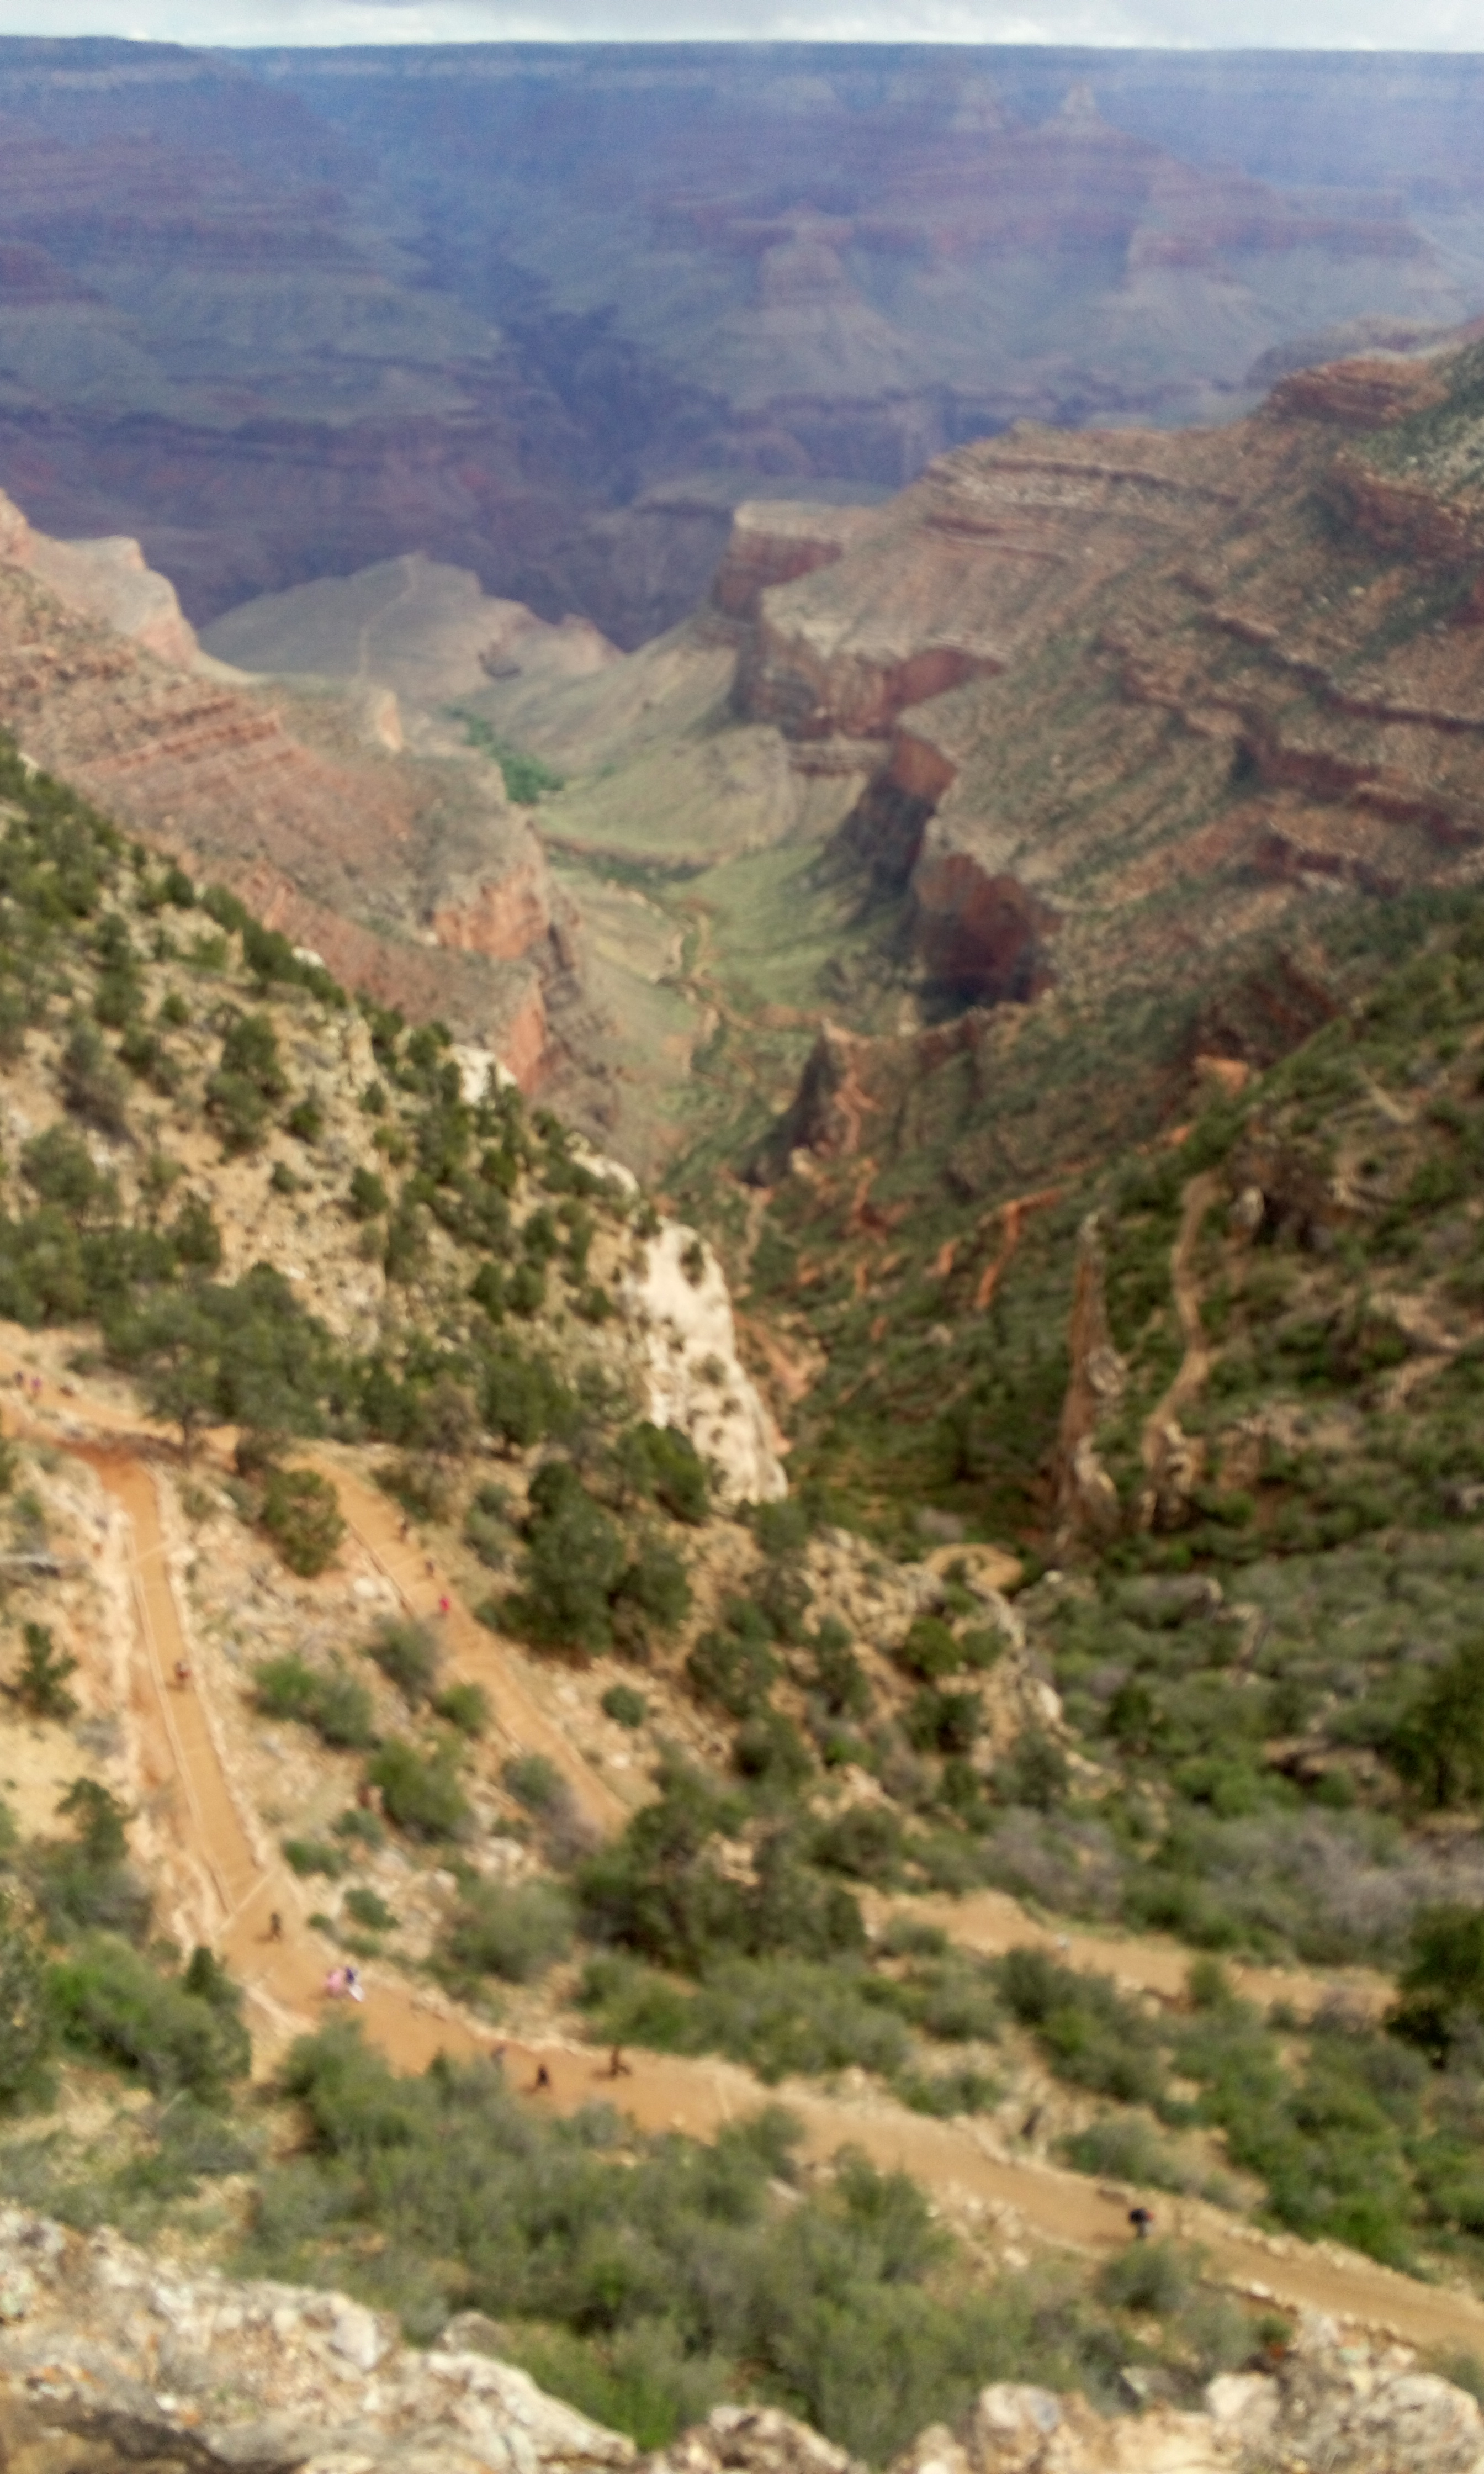
\includegraphics[width=\paperwidth,height=\paperheight]{10/image20160410_120920455.jpg};%
};
%  \node[black,fill=white,text width=10em] (blub) at (0.5,0) {Distanz etwa 3.600~km}; %
\end{tikzpicture}
\newpage

Beeindruckt vom Grand Canyon ging es am Nachmittag weiter zum nächsten Staudamm, dem Hover-Damm.
Wir kamen jedoch recht spät an und zu dieser Zeit war es untersagt den Damm zu Fuß zu betreten.
So ging es die überschaubar vielen Meilen noch nach \TOWN{Las Vegas} weiter.\\

Ich hatte ein paar Lichter in Form von Neonröhren erwartet, aber \FOREIGN{The Strip} ist mehr als nur ein paar Lichter.
Nachdem wir ins \FOREIGN{Treasure Island} eingecheckt hatten, sind wir am sehr späten Abend nochmal losgelaufen, um etwas zu essen.
Am \FOREIGN{Strip} finden sich in erster Reihe hauptsächlich Hotels, aber hier und da gibt es auch etwas Gastronomie.
Neben dem goldenden M fand sich ein mexikanischer, ein chinesischer und ein Pizza-Imbiss.
Selbstverständlich ist man offen für alles, doch dann fällt einem wieder ein, dass man im Heimatland stellenweise schon größte Probleme hat beim \glqq Ausländer\grqq \, etwas zu bestellen und dann auch noch das zu bekommen, was man wollte.
Folgerichtig gab es daher Pizza.
Calzone Meatball und Calzone Chesse.
Pizza zum Abgewöhnen.


\subsection*{Vasensaufen!}


\thispagestyle{empty}
\begin{tikzpicture}[remember picture, overlay]
\node[inner sep=0pt, xshift=.25\paperwidth, yshift=.25\paperheight] (vase) at (current page.south) {%
	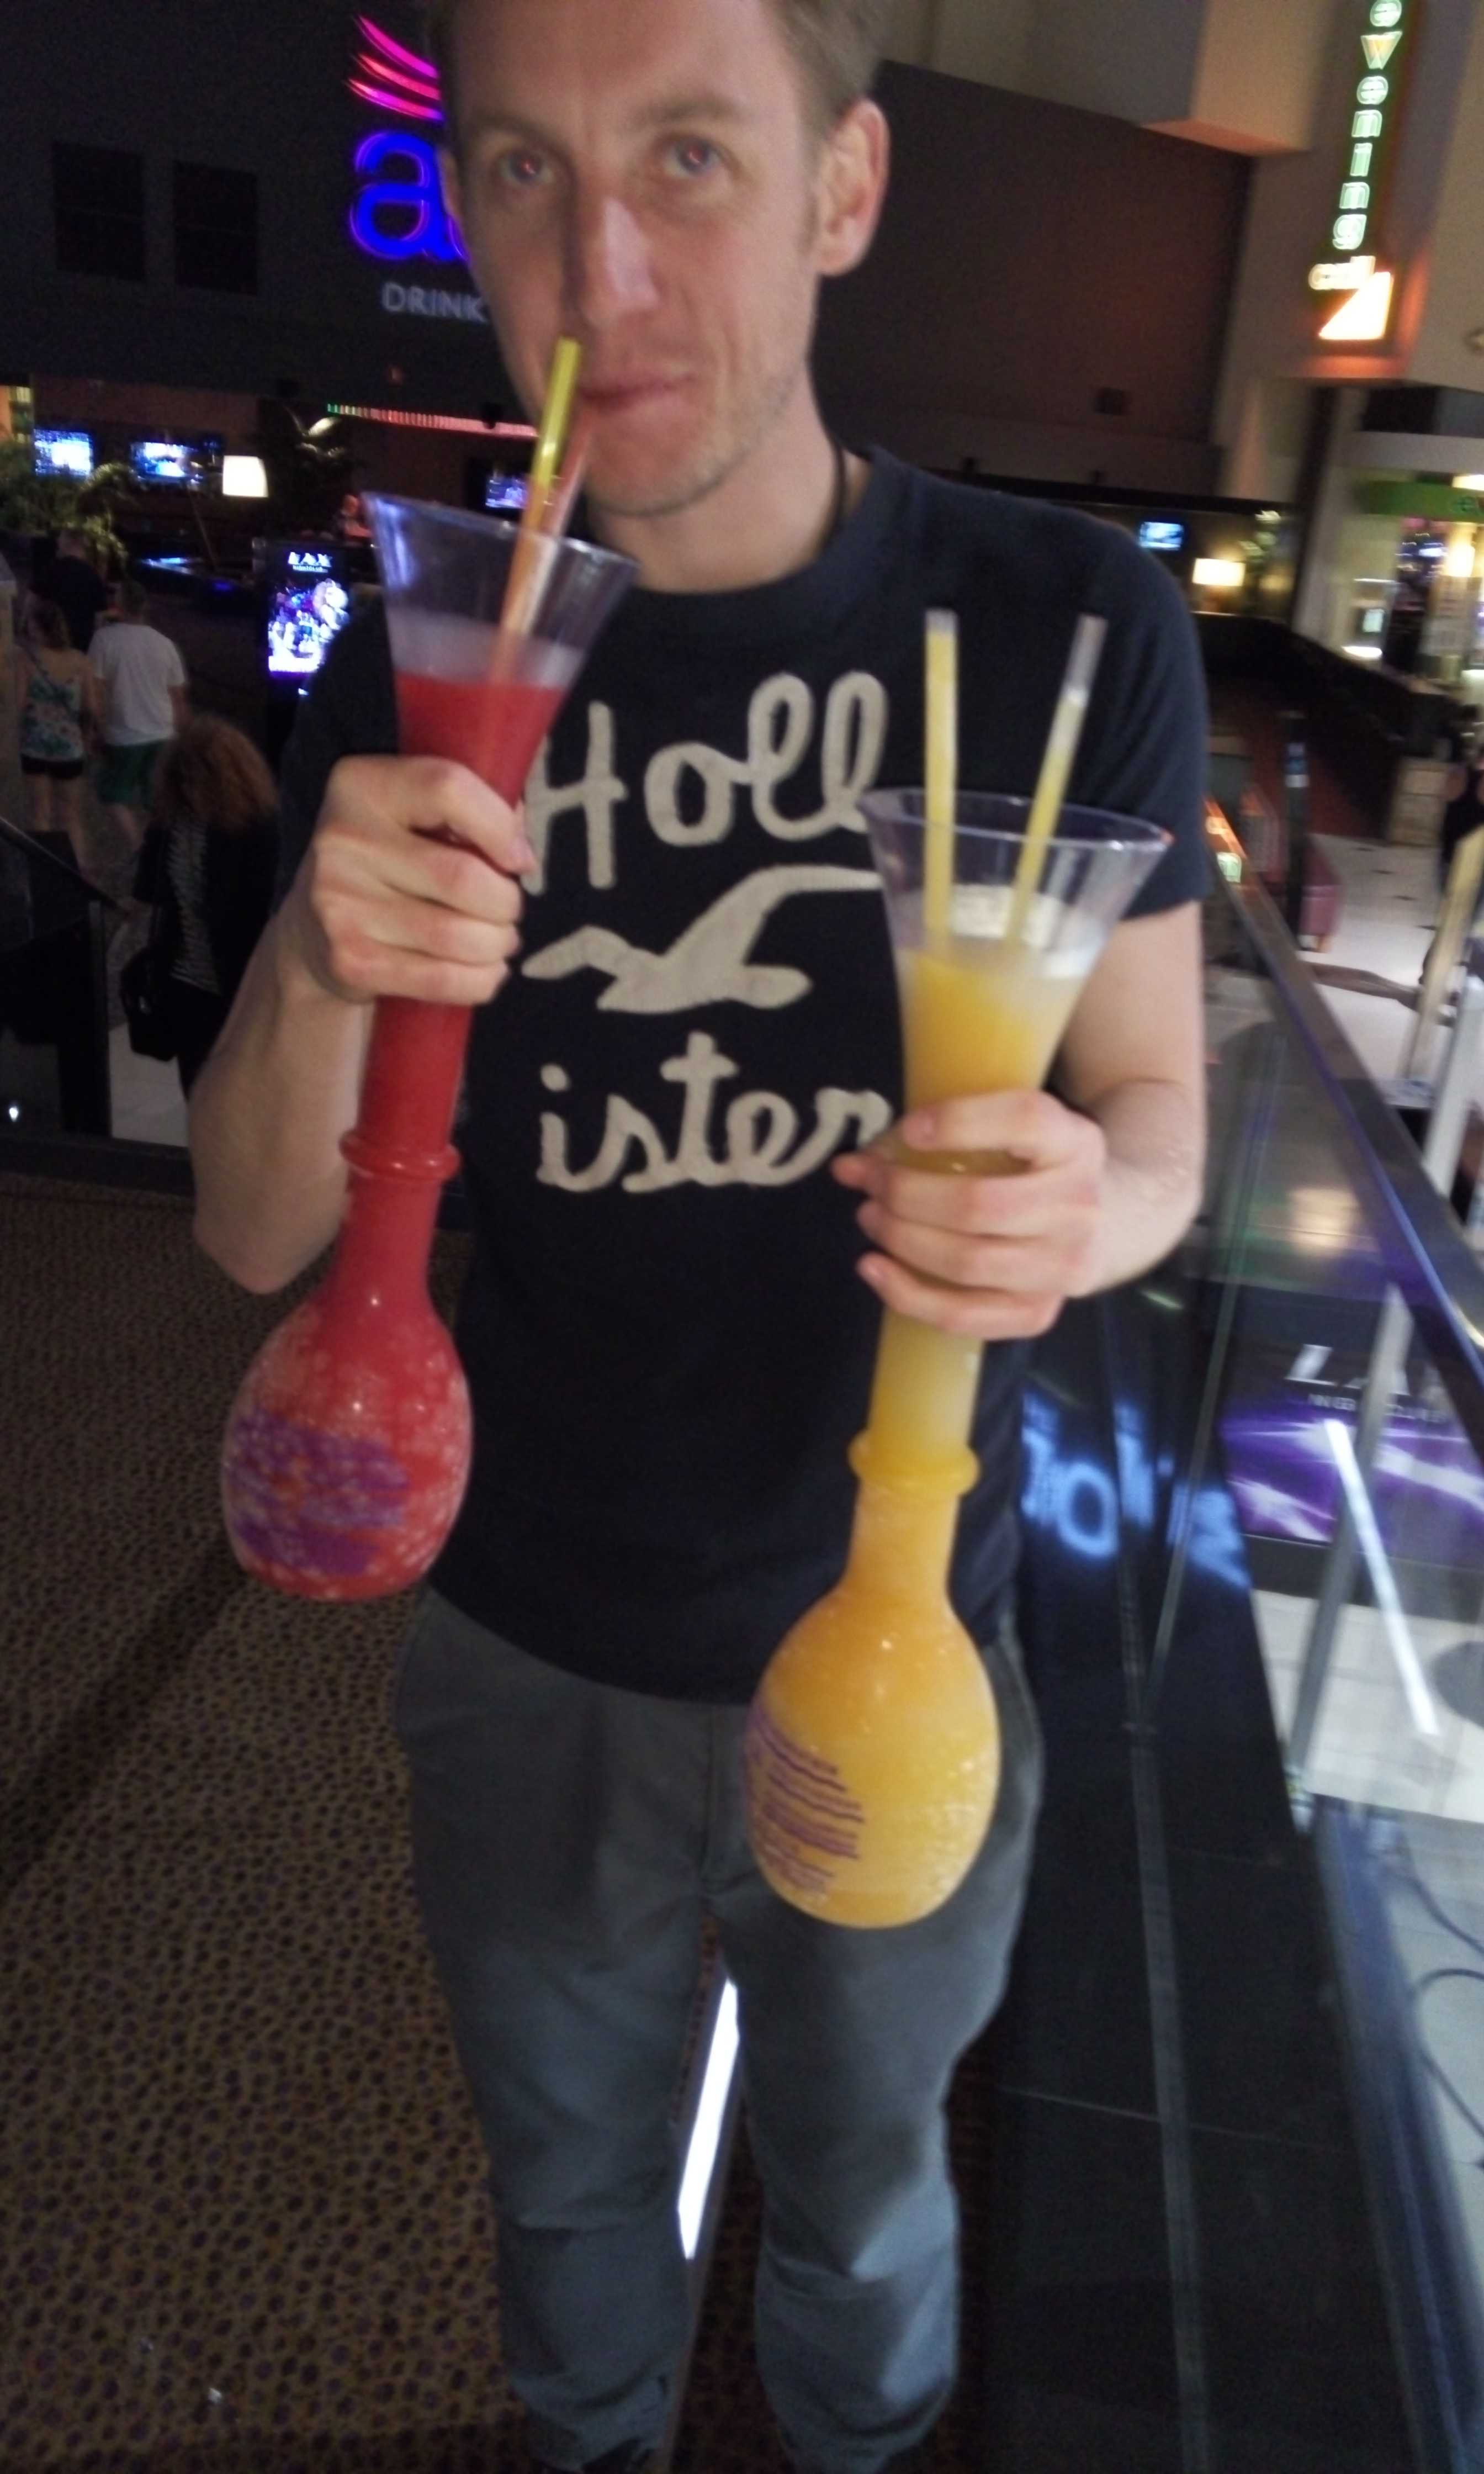
\includegraphics[width=.5\paperwidth,height=.5\paperheight]{11/image20160411_134402409.jpg};%
};
\node[inner sep=0pt, text width=.35\paperwidth, align=justify, xshift=-.2\paperwidth, yshift=1.2cm] at (vase.west) {%
	\FOREIGN{The Strip} war das Tagesprogramm.
	Den Boulevard sind wir auf der einen Seite hoch und auf der anderen Seite, mit ein bis zwei Vasen intus in leicht beeinflusster Gangart, wieder herunter gelaufen.
	Die einzelnen Hotels haben verschiedene Mottos und jedes ist dann doch irgendwie beeindruckend!
	
	Wenn man dann weiß, dass der Großteil der Hotels dem Hollywood Filmstudio MGM gehört, erscheinen die hier spielenden Filme (Ocean 11\dots 13, Hangover 1\dots 3, \dots) in einem anderen Licht.
};
%  \node[black,fill=white,text width=10em] (blub) at (0.5,0) {Distanz etwa 3.600~km}; %
\end{tikzpicture}

\newpage

%\vspace*{1cm}

Der Vaseninhalt ist alkoholhaltiges Squash-/Wassereis und besteht in erster Linie aus billigstem Fusel.
Vom vielen Laufen und anderem sind wir gegen Abend angeknockt mal kurz ins Bett gefallen und nach zwei statt der vorgenommenen einen Stunde unter größter Überwindung wieder aufgerumpelt.
Wir wollten noch etwas Essen und das beim Herumlaufen gefundene \FOREIGN{BeerHaus} klang vielversprechend.
Das Essen war weder berauschend noch gut, es füllte nur den Magen.
Die Wirkung der Vasen setzte uns weiterhin kräftig zu und wir liefen zurück ins Hotel.

Auf dem Heimweg wurde uns noch Coke angeboten, aber zu dem Zeitpunkt hatten wir beide schon die Schnauze voll von Gesellschaftsdrogen.
Ein anderer Geschäftsmann sprach uns noch wie folgt an.
\begin{quote}
	\FOREIGN{Want some titties tonight?}
\end{quote}
Was ich verneinte und er daraufhin sein Angebot erhöhte.
\begin{quote}
	\FOREIGN{They are wrapped in bacon!}
\end{quote}
Zu seinem Pech kamen wir gerade vom Essen und wollten nur noch irgendwie durch den aus Spielautomaten und -tischen bestehenden Irrgarten im Erdgeschoss unseres Hotels.


\subsection*{Palm Springs}
Mit wahnsinnigen Kopfschmerzen unerklärlichen Ursprungs haben wir Las Vegas in Richtung Süden verlassen.
Auf dem Weg nach \TOWN{Palm Springs} liegt der National Park Joshua Tree, eine Wüste.
Gefrühstückt hatten wir in einem Diner für weniger als die Hälfte verglichen mit dem Frühstück vom Vortag.
Gut gestärkt, eher überfressen, ging es zurück auf die Straße wobei ich zum ersten Mal das Steuer übernahm.
Das Fahren hier ist etwas anders als daheim. Es gibt kein rechts vor links, sondern wer zuerst kommt mahlt zuerst.
Ebenso gibt es kein Rechtsfahrgebot, dadurch kann rechts wie links überholt werden und noch gravierender, auf dem Highway (Freeway?) gibt es Kreuzungen (X-ING = "Crossing") sowie Ampeln.
Die Geschwindigkeitsbeschränkung findet man sehr schnell angenehm, denn Überholmanöver sind dadurch sehr stressfrei und im Generellen muss man keine Bedenken haben, dass jemand von hinten angerauscht kommt.
Stellenweise lässt die Verfassung der Straße auch keine hohen Geschwindigkeiten zu.

Im Vergleich mit dem Grand Canyon ist der Joshua Tree National Park erstmal nicht so beeindruckend, aber auf eine andere Art doch ganz hübsch.
Vor allem ist es dort ruhig, weil weniger besucht.
Die angefahrenen Aussichtsplattform (Keys West) war zwar ein voller Reinfall, aber die auf dem Weg gelegenen Spots waren recht nett.
Denn diese bestanden i.d.R. aus Felsen, auf denen man herum klettern konnte und die waren wahnsinnig griffig!

\newpage
\thispagestyle{empty}
\begin{tikzpicture}[remember picture, overlay]
\node[inner sep=0pt, yshift=-.25\paperheight] at (current page.north) {%
	\includegraphics[width=\paperwidth,height=.5\paperheight]{12/image20160412_170805538.jpg};%
};
\node[inner sep=0pt, yshift=.25\paperheight] at (current page.south) {%
	\includegraphics[width=\paperwidth,height=.5\paperheight]{12/image20160412_164403875.jpg};%
};
\end{tikzpicture}
\newpage

Auf dem Weg nach \TOWN{Palm Springs} lagen dann noch ein paar tausend Windräder\dots
Der Ort selbst war dann im Endeffekt nur eine lang gezogene Hauptstraße mit Palmen.
Wirklich nicht der Rede wert.


\subsection*{San Diego}
Ich habe keine Ahnung wie der Christian bei dem konstanten Lärm- nicht nur Geräuschpegel, Lärmpegel ohne Ohrstöpsel überhaupt ein Auge zumachen konnte.
Vielleicht trug das griechische Abendessen seinen Teil dazu bei, aber ausgeschlafen und fit sieht ganz anders aus.
Wir sind dann erstmal zum Walmart, um - zusammengefasst - Schrott zu kaufen.
Wasser war auch dabei sowie unser Frühstück bestehend aus Toastbrot und Käse, aber alles andere war nur Schrott.
Die Kekse mit Schokostücken, wie es sie bei uns auch gibt, waren noch okay, der 5Gum-Kaugummi mit Geschmacksrichtung Peppermint schmeckt nach Zahnarzt und die Schnüre waren ungenießbar.
Unsere anschließende Suche nach einem At\&t Geschäft verlief erfolglos und so fuhren wir ohne Möglichkeit online zu buchen gen San Diego.
Auf dem Weg dahin standen nicht nur ein paar Windräder sondern hunderte.
Diese waren nicht so groß wie zuhause, dafür dichter zusammengepackt.

Das letzte Stück bis San Diego auf dem sechs oder gar acht spurigen Freeway war dann alles andere als ein Zuckerschlecken.
Die Ansage des Navis "Folgen Sie den linken Spuren" stand unserem Wunsch möglichst rechts zu fahren, um die richtige Ausfahrt nicht zu verpassen, deutlich entgegen.
In den Hafen (Downtown) schafften wir es dann letztlich doch irgendwie und dort setzten wir nach einer kurzen Hafenbesichtigung unsere Suche nach einem At\&t Shop fort.
Gefunden haben wir auch einen, wir waren wieder online (Guthaben aufgeladen) und konnten uns so der Suche nach einer Unterkunft widmen.
Hotels gab es natürlich auch, doch das Hostel war deutlich billiger, vor allem weil beim Hotel auch kein Parkplatz mit enthalten war.

Tagsüber stolperten wir im Hafen herum, am Abend wollten wir uns den "berühmten" Zoo bzw. das Drumherum anschauen.
Den Zoo haben wir nicht so recht ausmachen können, aber der Balboa Park indem der Zoo eingebettet ist, ist selbst eine ganz schöne Parkanlage.
Diese befand sich mitten in der Einflugschneise des Flughafens.
In dieser Anlage befand sich ebenfalls ein Militärkrankenhaus sowie eine Schule.
Wo lernt es sich schließlich besser als in der Einflugschneise eines Flughafens?

Das Abendessen war dann wieder nur flüssiger Natur, da die Küche kurz vorher geschlossen hatte.


\subsection*{Kulturschock!}
Von San Diego kommt man mit der Straßenbahn bis zur mexikanischen Grenze und da wollten wir hin.
Doch davor stand erst der Gang zur Post an, denn der Christian musste noch etwas verschicken.
Es ging um Post ins Ausland, die fristgerecht ankommen musste.
Das trieb das Porto deutlich in die Höhe.
Aus ein paar Dollar wurden so 60 und mehr.
Nachdem sich der Christian für die Zustellung in 3-5 Tagen entschieden und das entsprechende Formular ausgefüllt hatte, wies ihn der Postbeamte Jesus darauf hin, dass er ein anderes Formular braucht.
Also das Ganze nochmal von vorne, wir kamen uns vor wie Asterix \& Obelix (bei der Götterprüfung im ??? TODO).

Eine gute Stunde später ging es dann zum Trolley (S-Bahn) weiter.
Ein Ticket hatten wir zwar beide gelöst, aber ob das auch gleich entwertet wurde, haben wir nicht begriffen.
Die Fahrt über waren wir daher leicht angespannt.
Daran änderten auch das komische Gebaren mancher mitfahrenden Frau nichts.
Eine sang leise, aber hörbar, vor sich hin.
Die nächste parfümierte sich und damit die halbe S-Bahn gleich mit und die letzte parfümierte ihre Handgelenke und drückte diese sogleich auf ihre Haare.

Der Grenzübertritt nach Mexiko war dann chillig.
Die Grenzpolizisten nahmen einem sogar die Arbeit ab, was das Ausfüllen der Unterlagen betraf.
Gleich nach Übertritt war es dann vorbei mit der chilligen Atmosphäre.
Alle 5~m hat uns ein Taxifahrer nach dem anderen angehupt, weil er uns in die Innenstadt fahren wollte.
Ich wollte aber laufen, was wir auch taten.
Den Weg wussten wir nicht, die am Straßenrand stehenden Taxifahrer waren aber auskunftsfreudig.

Vorbei an Werbeplakaten für schöne Zähne ging es über eine Brücke in die Innenstadt.
Das hektische Treiben und vor allem die schon wieder leicht anderen Verkehrsregeln ließen unseren Adrenalinspiegel gut ansteigen.
Unterm Strich sind wir die Straße einmal hoch und wieder runter gelaufen.
Um dann letztlich in der nicht sonderlich mexikanischen Touri-Bude amerikanische Preise zu zahlen.

Für uns war das dann erstmal genug Kulturschock und nachdem uns die Rezeptionistin vom Hostel gestern kräftig Angst gemacht hatte, wollten wir auf jeden Fall deutlich bevor Einsetzen der Dunkelheit wieder zurück sein.
Am Grenzübergang standen wir dann eine gute Stunde an, unterhielten uns mit einem Mexikaner, der schon seit längerem in den USA wohnt und zum Kauf von "Medikamenten" öfters in seine Heimat reist.
Er empfahl uns ein paar Flecken in L.A. unserem nächsten Ziel.


\subsection*{Zu den Engeln}
Ausgecheckt und den beim ersten Hafenrundgang entdeckten Flugzeugträger USS Midway angefahren.
Vor Ort haben wir ein Parkuhrticket für $1 \frac{1}{2}$ Stunden gelöst, weil ich der Über\-zeugung war, dass das Ding bestimmt nicht mehr hergibt.
Denkste.
Auf dem Flugdeck alleine steht genug Material in Form von Hubschraubern und Kampfjets für eine gute Stunde herum.
Unter Deck sind wir durch die Schlafkabinen der Mannschafter und Offiziere sowie den \FOREIGN{Ready Room}\footnote{Einsatzbesprechungsraum} spaziert.
Sämtliche Abzweigungsmöglichkeiten sind ab- bzw. versperrt, in dem Labyrinth soll sich schließlich niemand verlaufen.
Unter Deck 

%\newpage
%\thispagestyle{empty}
\begin{tikzpicture}[remember picture, overlay]
\node[inner sep=0pt, yshift=-.2\paperheight] at (current page.north) {%
	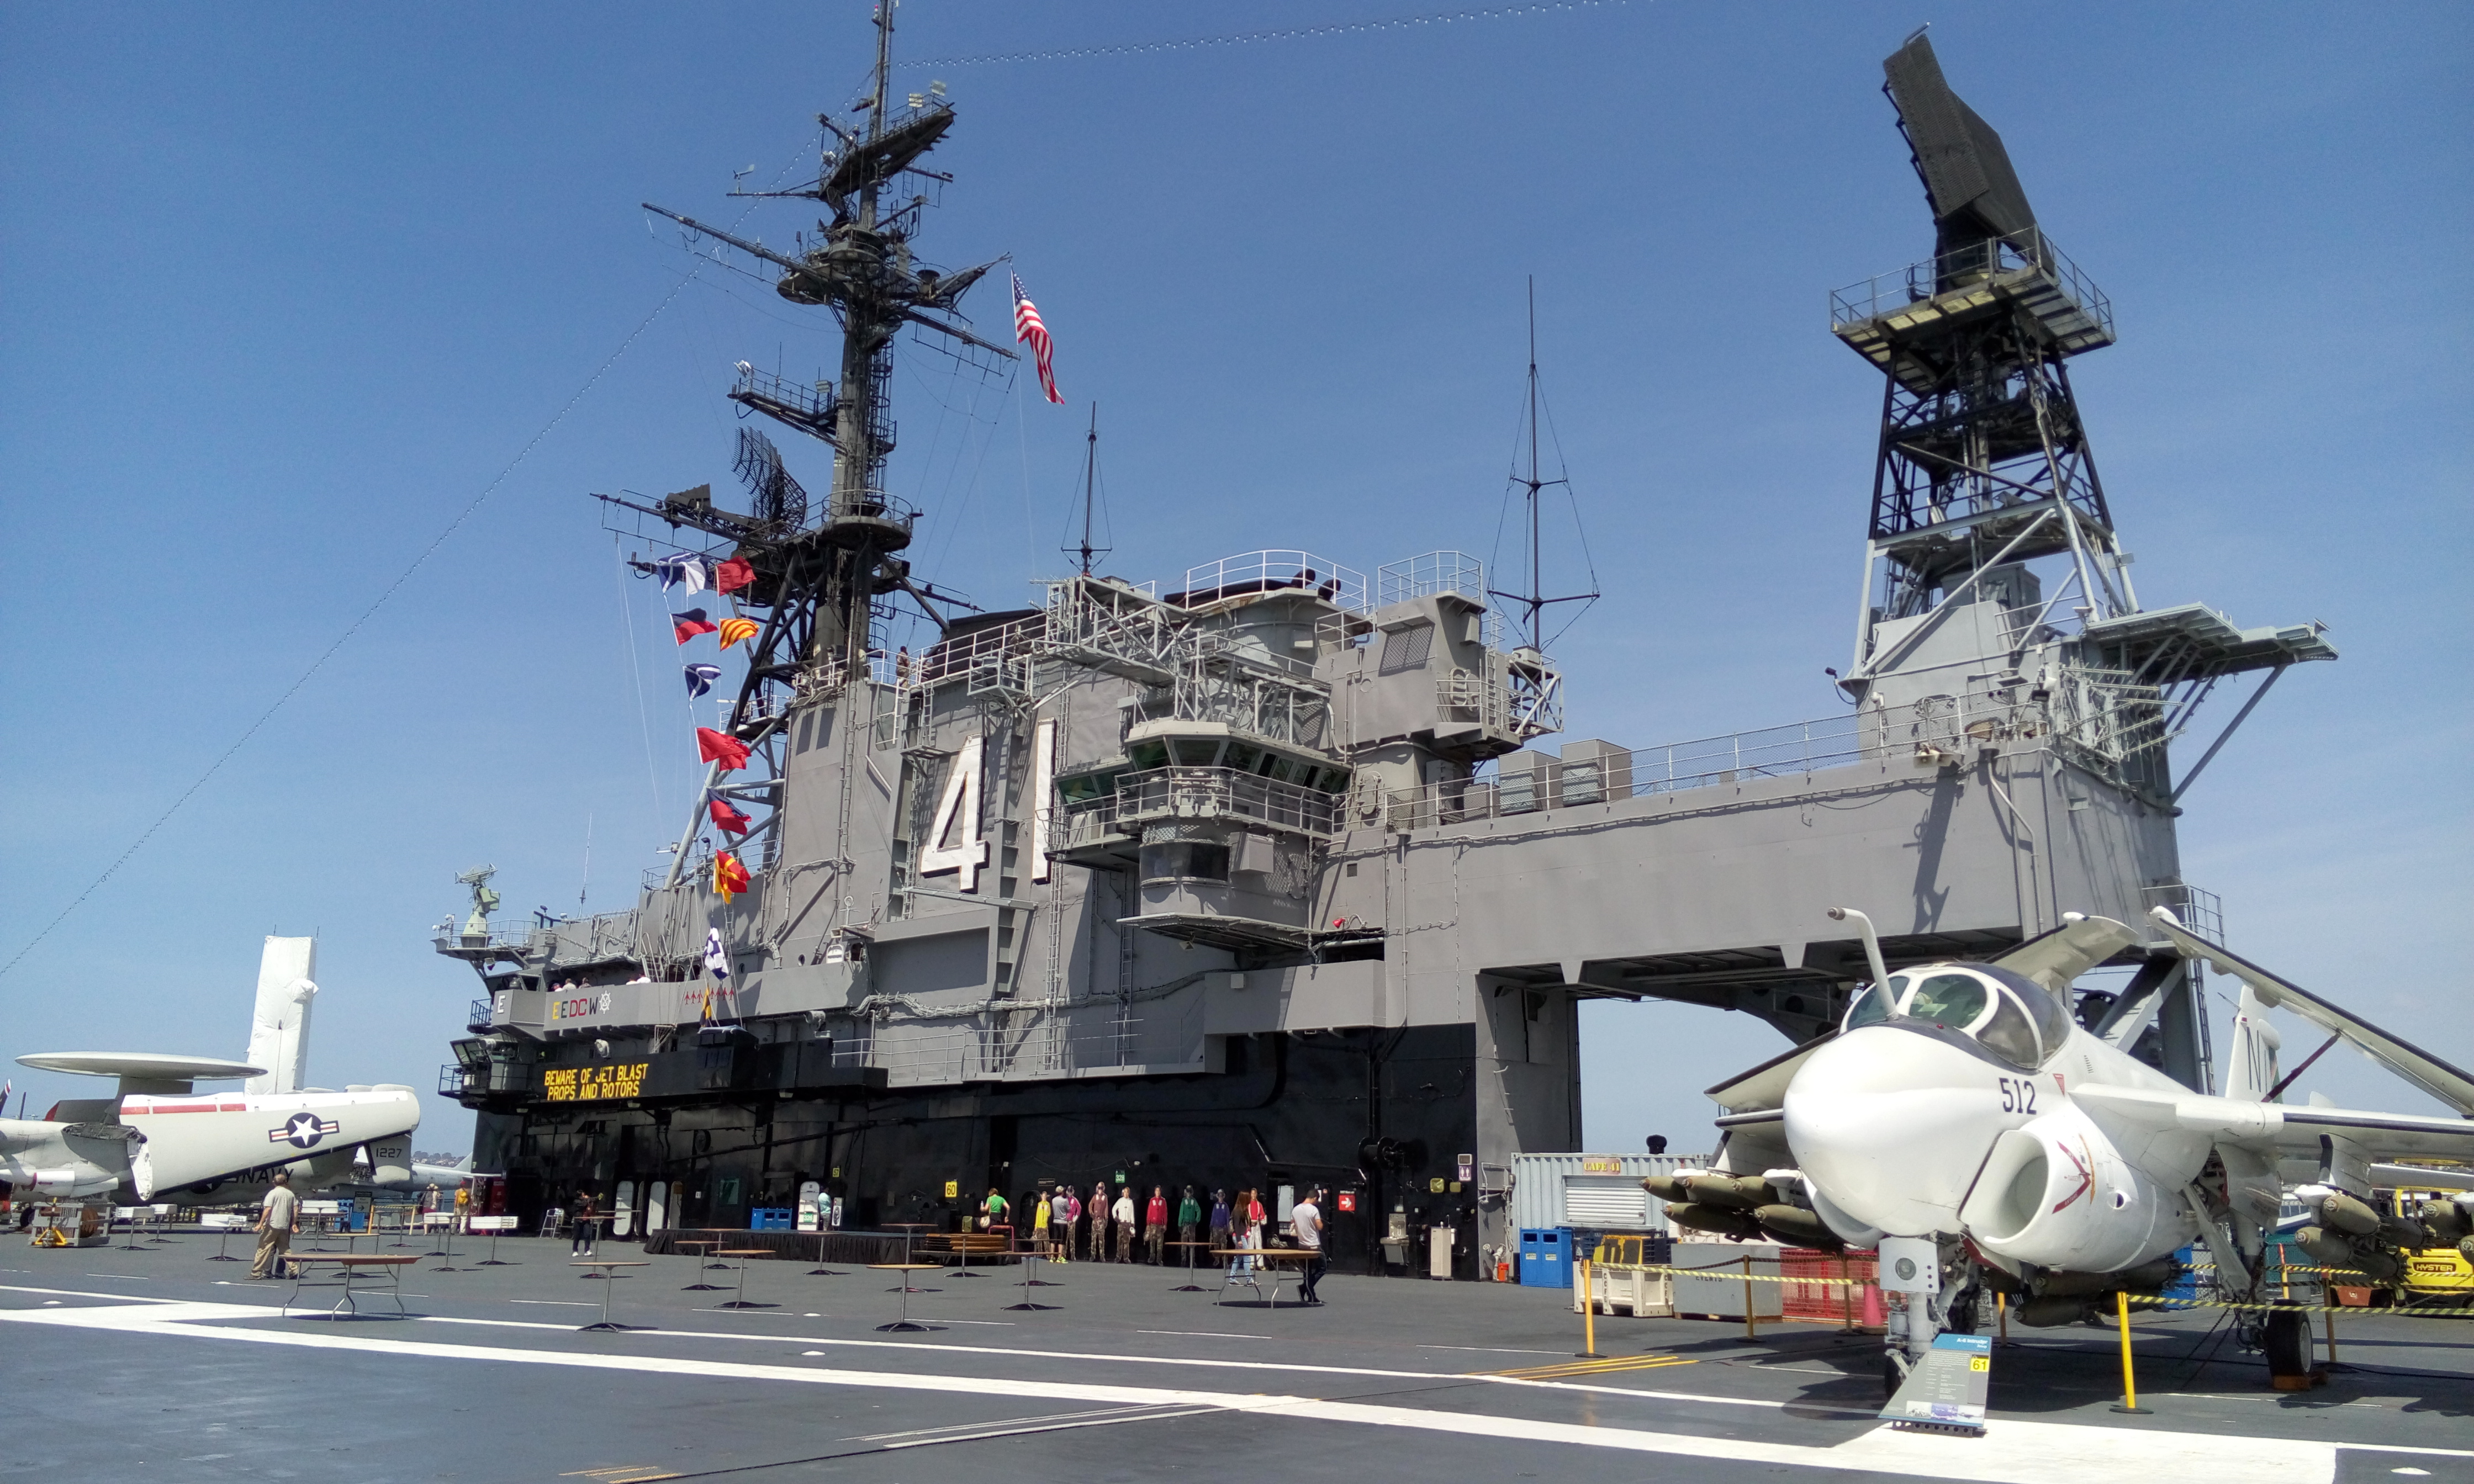
\includegraphics[width=\paperwidth,height=.4\paperheight]{15/image20160415_114740885.jpg};%
};
%\node[inner sep=0pt, yshift=.25\paperheight] at (current page.south) {%
%	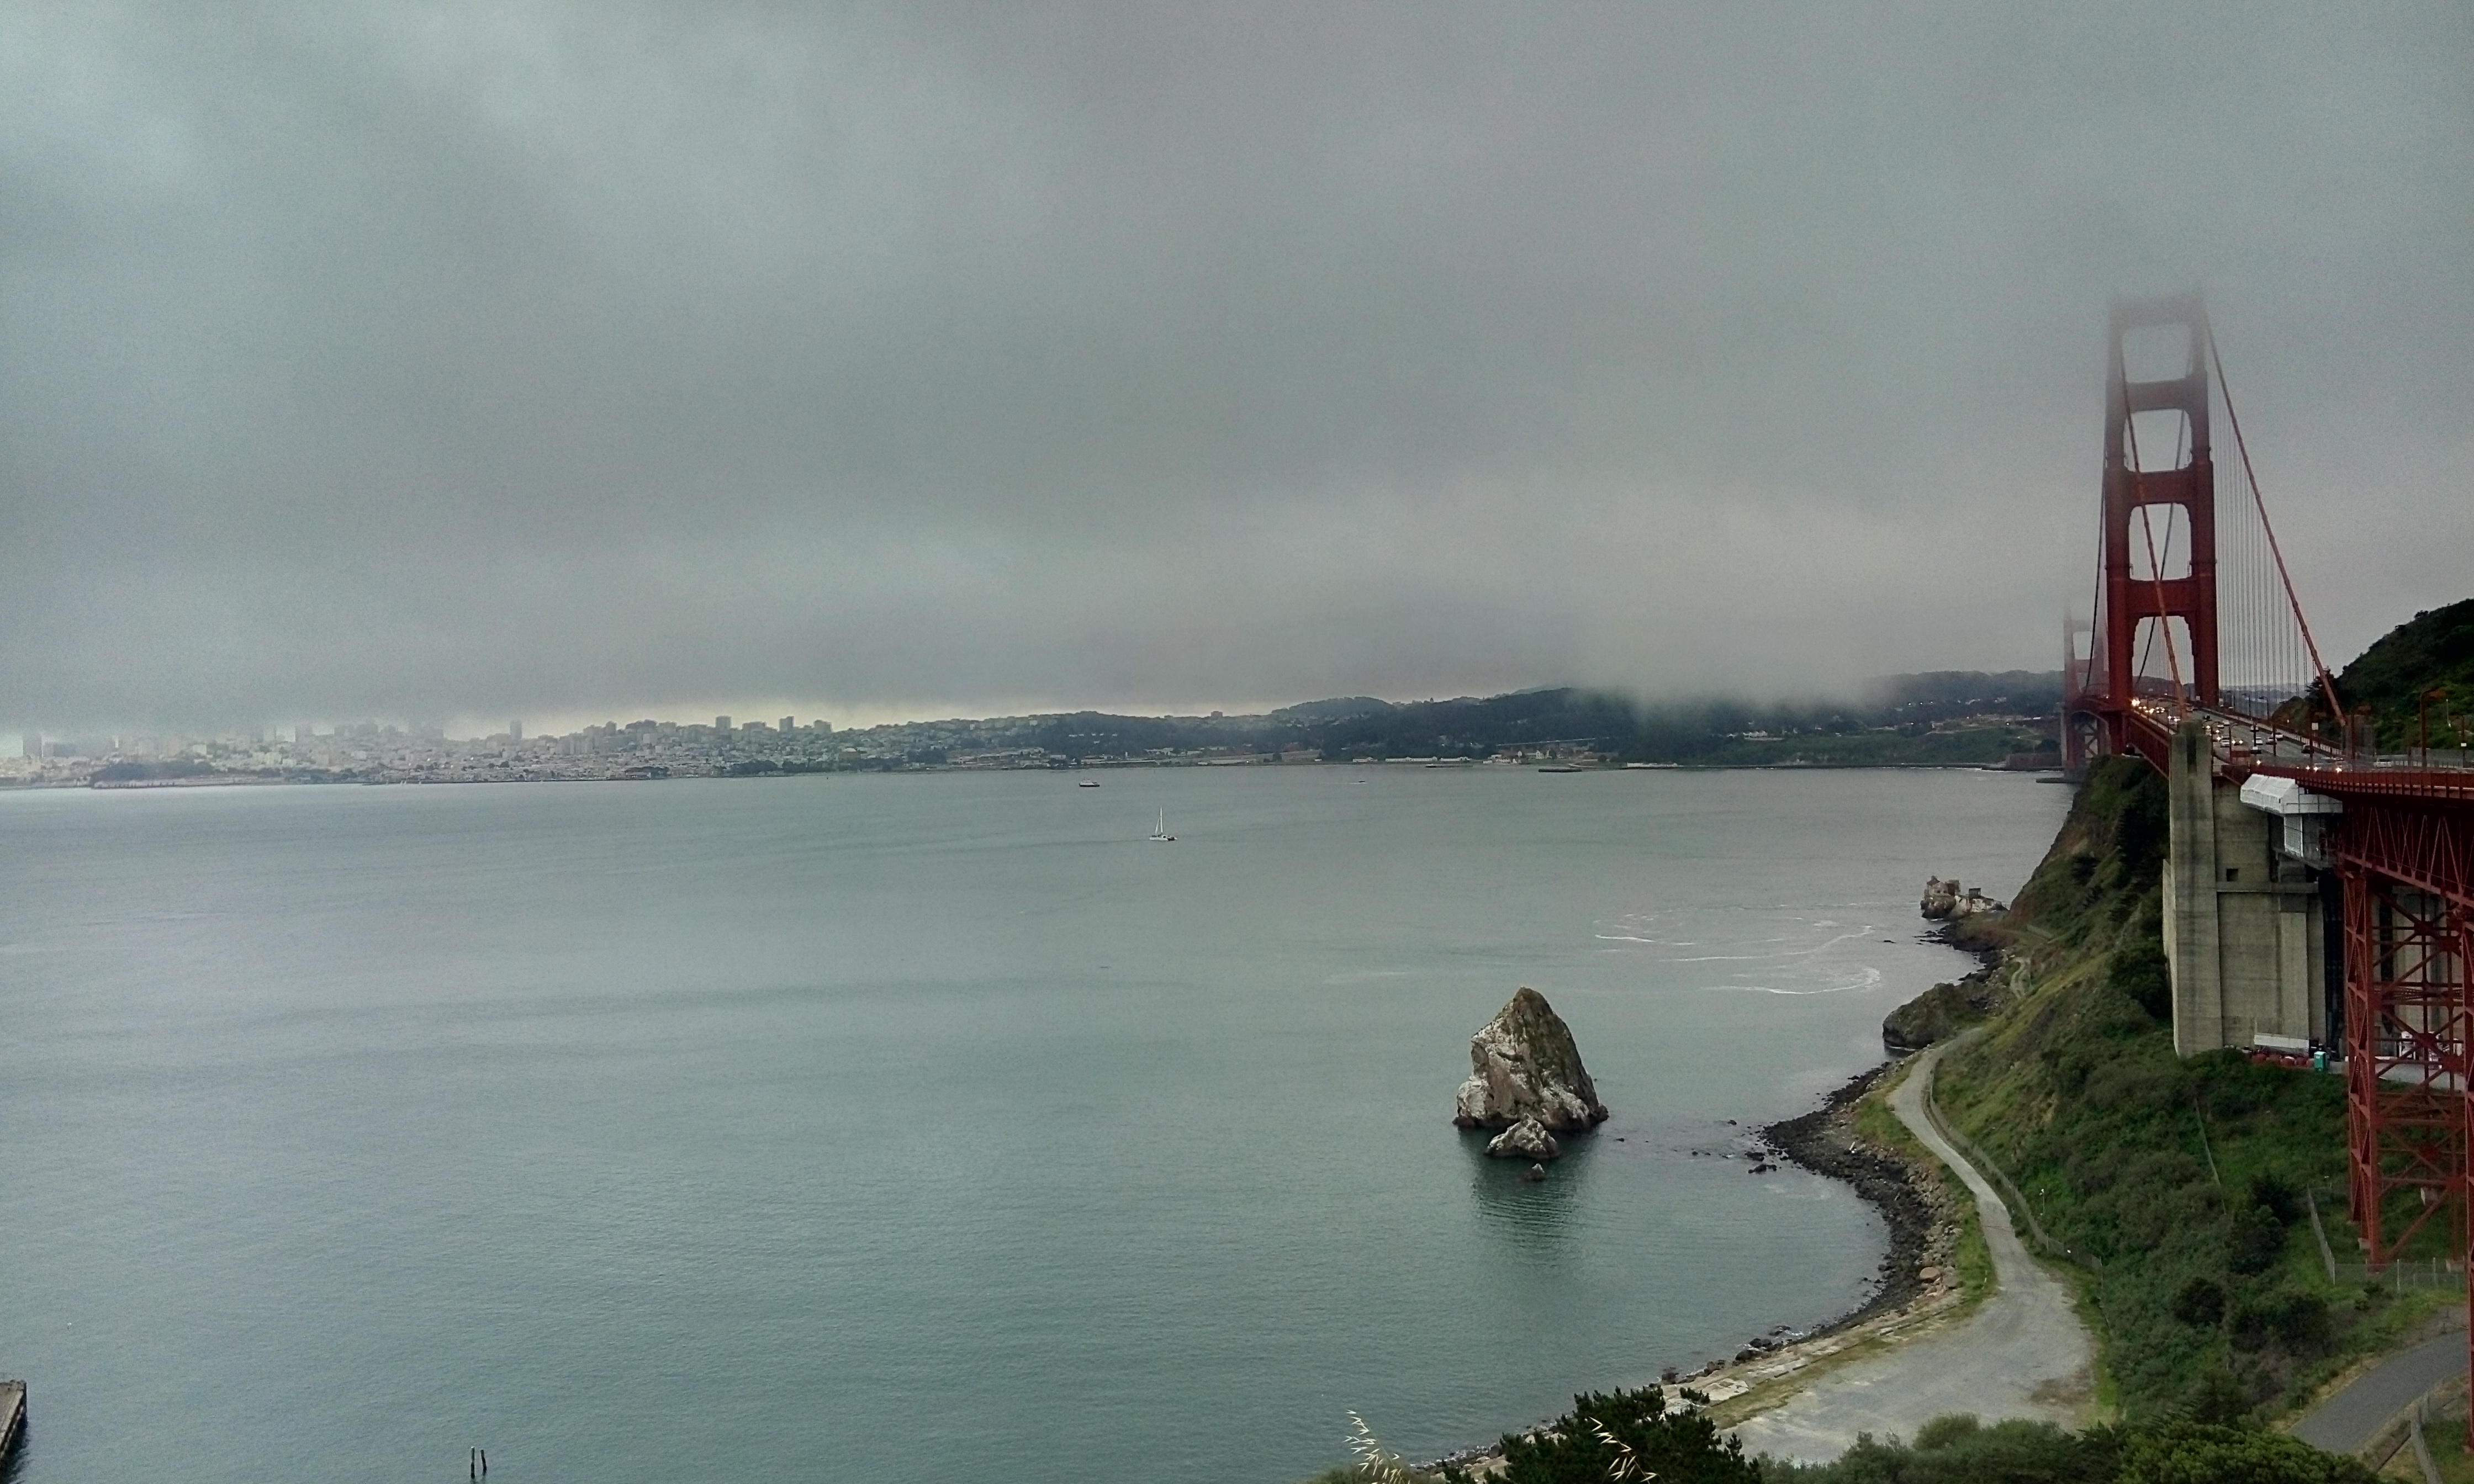
\includegraphics[width=\paperwidth,height=.5\paperheight]{21/image20160420_193101911.jpg};%
%};
\end{tikzpicture}

\vspace*{.3\paperheight}

\noindent
Deck gab es auch ein paar spaßig wirkende Flugsimulatoren, für die wir leider keine Zeit hatten.
Erst recht nicht für den Maschinenraum.

Die Parkuhr war bei unserer Rückkehr gut abgelaufen und dann ging es auch schon weiter in Richtung \TOWN{Los Angeles}.
Auf den \FOREIGN{Interstates}\footnote{Autobahn} hätte die Fahrt rund $2 \frac{1}{2}$ Stunden gedauert.
Über die gewählte \glqq historische\grqq \, \FOREIGN{Route 101} erreichten wir nach nur 6~Stunden unser Ziel.
Wir zogen die langsame Strecke der schnelleren vor in der Hoffnung so nicht wieder auf einer achtspurigen Straße zu landen.
Das war dann auch der Fall, mehr wie vier Spuren mussten wir nicht meistern.
Außerdem kamen wir so an Walen vorbei.

Für die kommenden Nächte ging es wieder ins Hostel.
Gebucht hatten wir ein 10er Zimmer, ein 8er bekamen wir und das war jede Nacht komplett belegt.
Trotz fluktuierender Kundschaft.
Mit den Übernachtungen im Hostel hatten wir gegenüber einem Hotel deutlich gespart und dann parkten wir das Auto noch für 5~\$ pro Tag statt 14~\$.
Deshalb ging es zum gehobenen Italiener.
Die Lasagne war ganz gut, die halbe Portion vom Christian ein Witz.


\subsection*{Stadtführung in L.A.}
Die Nacht im belegten 8~Mann Zimmer war in Ordnung, zumindest für mich.
Der Christian hat mit dem ersten Wort über seine Rückenschmerzen geklagt, was für ein Lappen.
Nachdem ich meinte, dass sich kaum einer gesund gelegen hat und er sich einfach bewegen soll, sank das Gejammer auf ein erträgliches Maß.
Das Frühstück war essbar und dann ging es zur Stadtführung.
Mit dem Linienbus ging es auf dem \FOREIGN{Interstate} für 30~Minuten Richtung \FOREIGN{Downtown}\footnote{Innenstadt}.
Dort angekommen führte uns unser obdachloser Stadtführer zur Stadtbibliothek, in ein Hotel, weil bei diesem die Aufzüge außen angebracht sind und man so die nähere Umgebung überblicken kann, in ein Büchergeschäft mit Künstlerateliers und zu einem Coffeeshop für einen kurzen Stopp.
Danach ging es weiter zum ehemaligen Bauernmarkt, der heute eine reine Fastfoodhalle ist, zur Disney Oper, nach \FOREIGN{Little Tokyo} und noch in ein mexikanisches Viertel.
Dort endete die anstrengende Rennerei.

Mit unseren neuen Bekanntschaften den Franzosen Maximili\textbf{e}n Ortiz und Pierre Bour (sie sind anschließend nach \TOWN{San Diego} weiter, um von dort den \FOREIGN{Pacific Crest Trail} zu laufen, was sie auch geschafft haben!), dem käsebleichen Hayden aus Manchester,

\begin{tikzpicture}[remember picture, overlay]
\node[inner sep=0pt, yshift=-.2\paperheight] at (current page.north) {%
	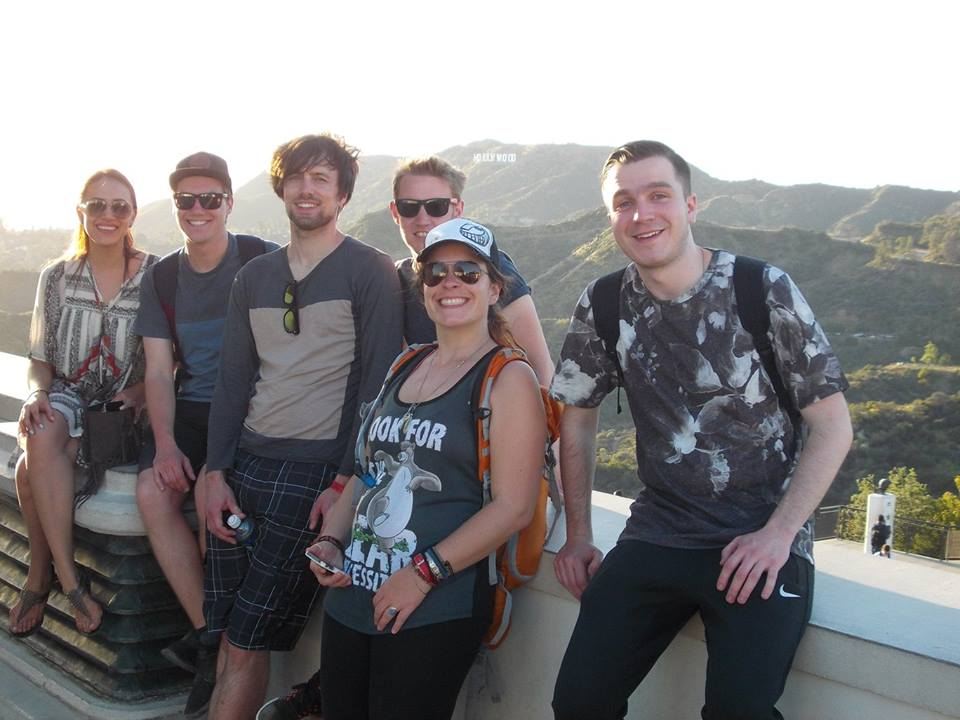
\includegraphics[width=\paperwidth,height=.5\paperheight]{16/la_gang.jpg};%
};
%\node[inner sep=0pt, yshift=.25\paperheight] at (current page.south) {%
%	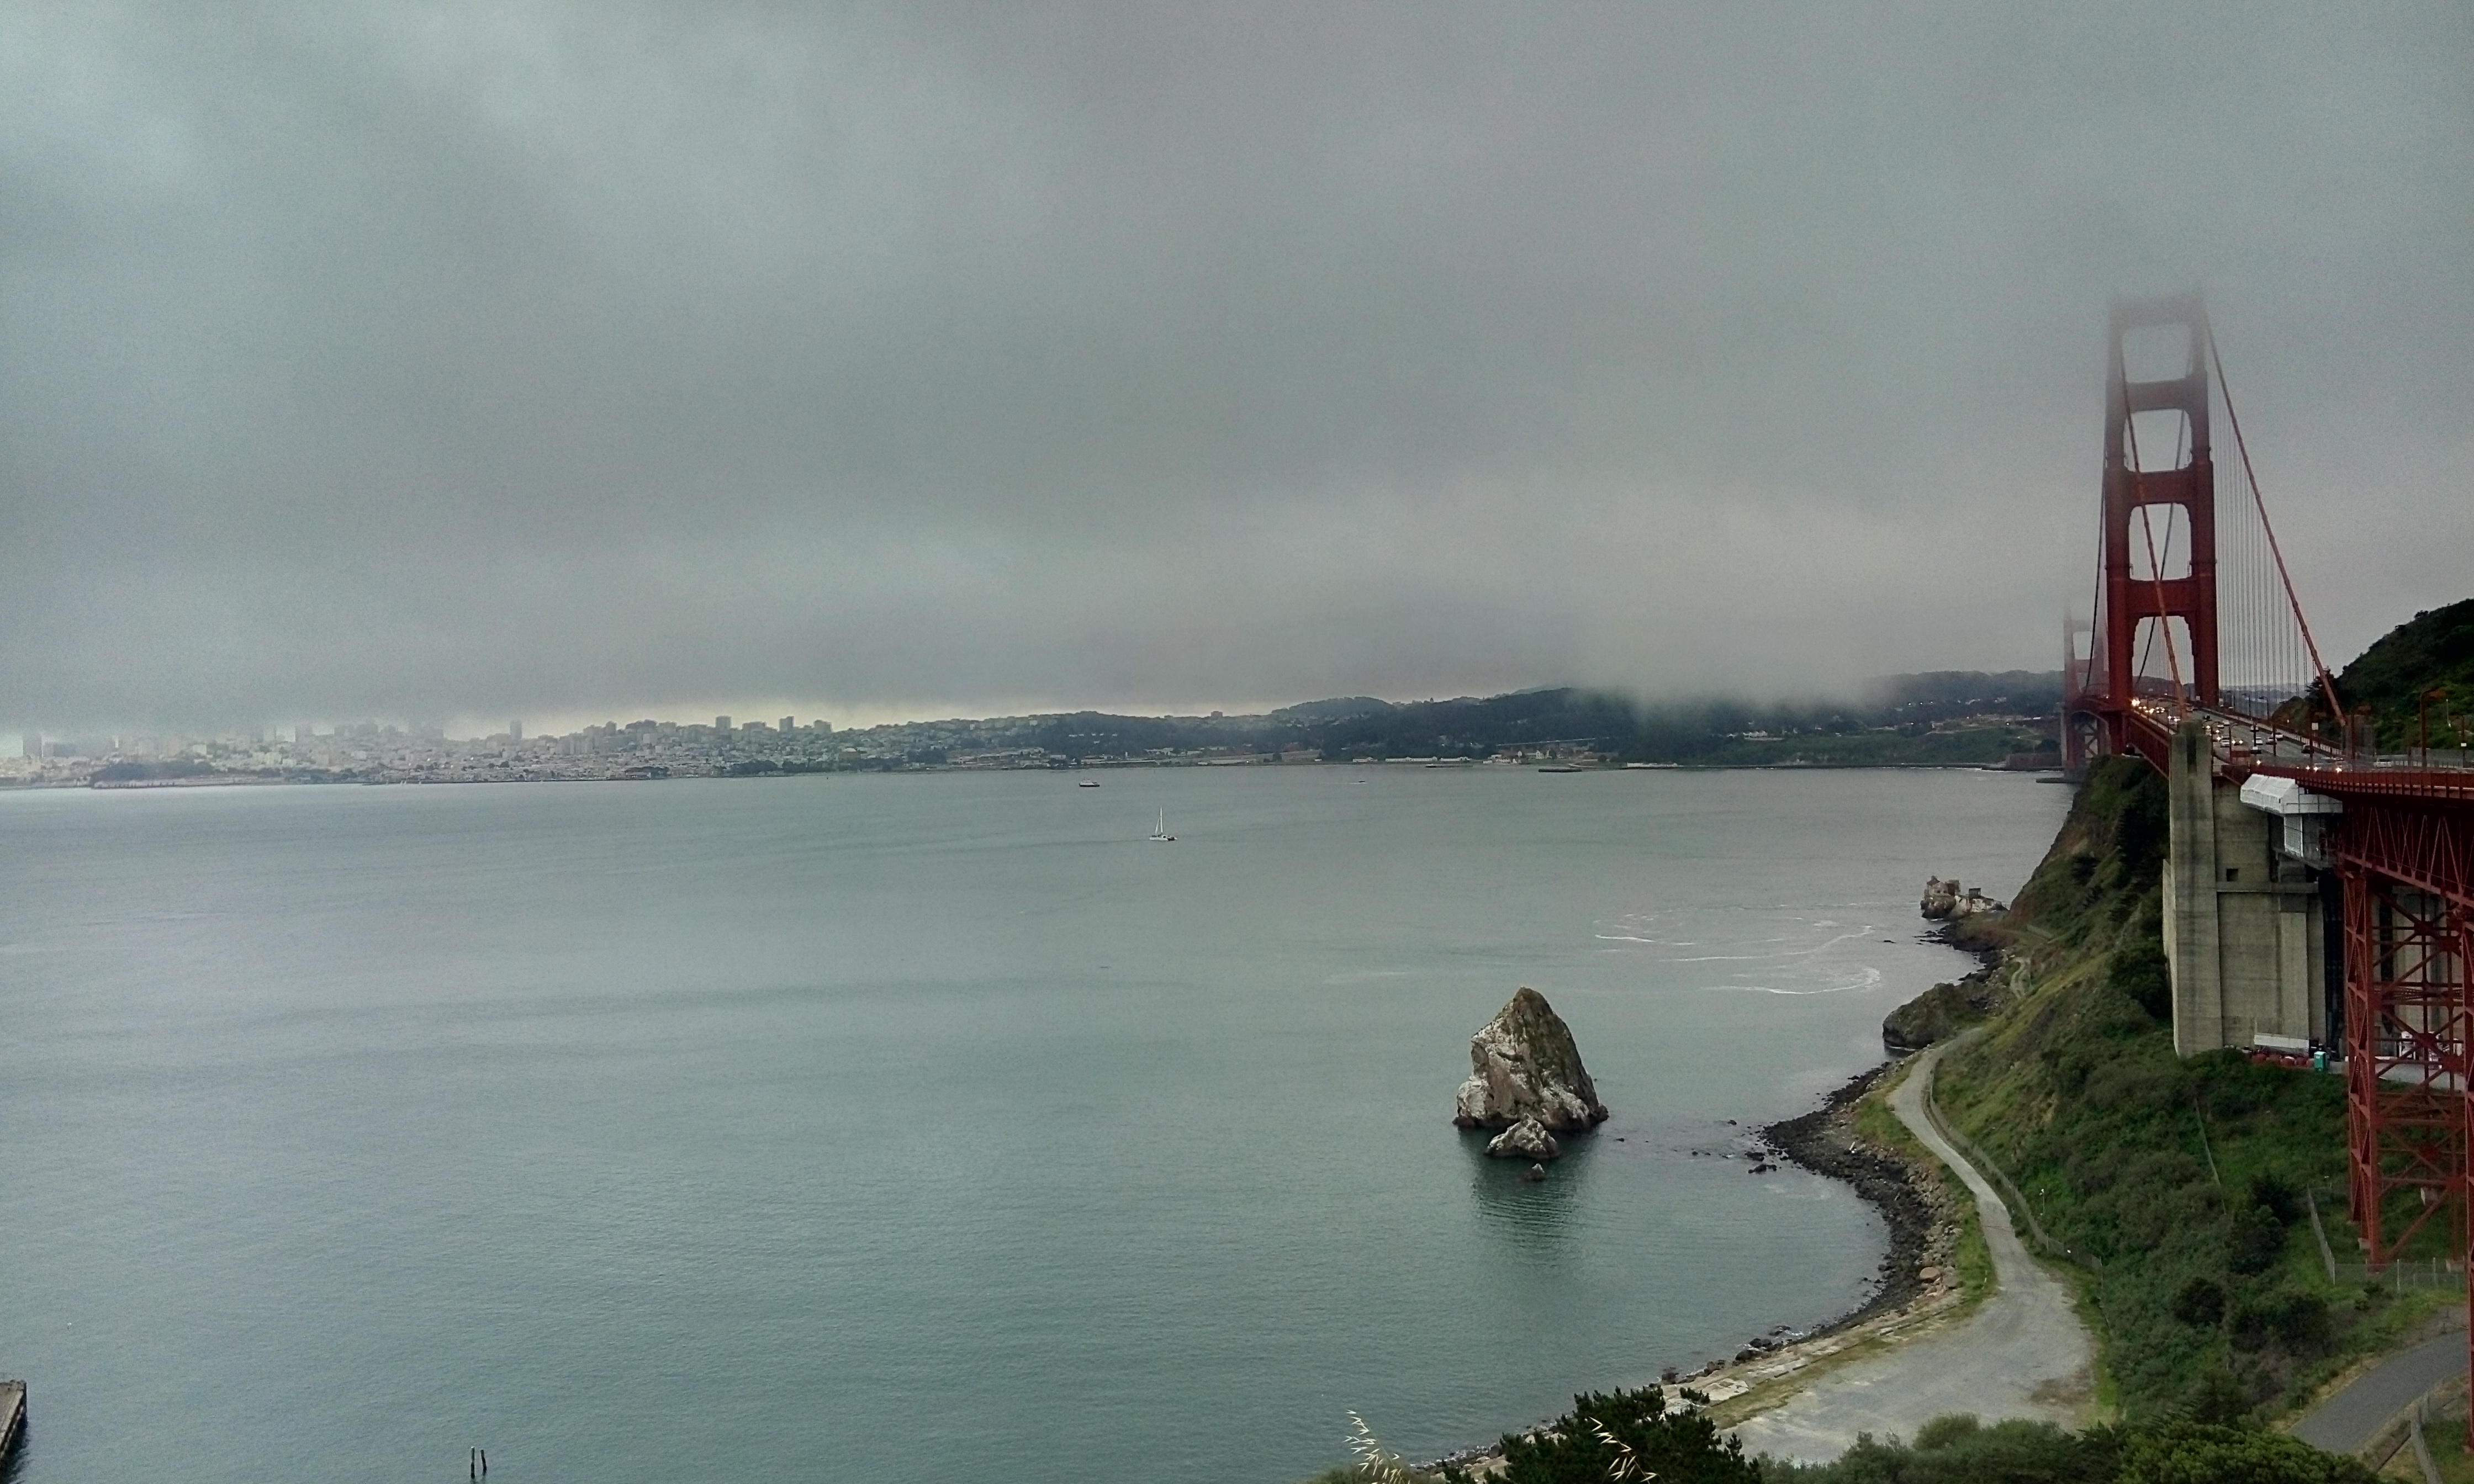
\includegraphics[width=\paperwidth,height=.5\paperheight]{21/image20160420_193101911.jpg};%
%};
\end{tikzpicture}

\vspace*{.3\paperheight}

\noindent
Manchester, der Weltreisenden Schweizerin Oona Baumier und der mexikanischen Mexikanerin Natalia Lopez ging es mit einer Uber-Fahrt zum Griffith \FOREIGN{Observatory}\footnote{Sternwarte}.
Zumindest in die Nähe.
Denn bis hoch ließen wir uns nicht fahren, das hätte 40~Minuten Stop\&Go bedeutet und wir gingen stattdessen zu Fuß.
Hayden wurde beim Aufstieg nochmals bleicher, weil er es nicht so mit engen, abschüssigen Trampelpfaden hat.
Mit Händchen halten haben wir ihn dann trotzdem hoch bekommen.
Das \FOREIGN{Observatory} hatten wir zwar knapp verfehlt, aber der angelaufene Hügel dahinter bot eh die bessere Aussicht.
Von dort aus hatte man auch eine gute Aussicht auf den berühmten Hollywood Schriftzug.

Von dort stiegen wir zum \FOREIGN{Observatory} ab, was wieder ein gewisses Drama bedeutete.
Wer was für unser Sonnensystem übrig hat, ist dort ganz gut aufgehoben.
Ich fand nur die Waagen zum Anzeigen des eigenen Gewichts (in lbs, also Pfund) auf dem jeweiligen Planeten ganz interessant.
Im Anschluss stand der richtige Abstieg an.
Da der Aufstieg in rund 20~Minuten möglich war, erwarteten wir eine ähnliche Zeit\dots es wurde allerdings eine gute Stunde.
Unten angekommen, dachten wir nochmal kurz über eine Uber-Fahrt nach, bis zur nächsten Bushaltestelle war es aber auch nicht weit.
Dort angekommen hatte sich der Uber-Preis bereits verdoppelt.
Ob es an der Anzahl verfügbarer Fahrer, der fortgeschrittenen Uhrzeit (es dämmerte bereits) oder der Gegend lag, lässt sich nur mutmaßen.
Der Bus kam dann und nach 50~Minuten waren wir am Hostel.

Von dort ging es mit nüchternem Magen zum nahegelegenen Pub \FOREIGN{``Ye Olde Kings Head''} auf ein paar Runden Bier.
Nach Runde drei verging mir der Durst, aber der Christian war auch nach Runde fünf derart unterhopft, dass er sich eines herrenlosen Bieres annahm.
Gegen 2~Uhr hat der Pub alle Gäste vor die Tür gesetzt und wir gingen heim, wovon Christian nichts mehr weiß\dots\\[1em]

\marginline{\texttt{Gegen\-dar\-stellung}}
\fbox{%
\parbox{.9\textwidth}{%
Es war kein \glqq herrenloses Bier\grqq\, sondern Thorstens.
Denn der war währenddessen sehr intensiv mit der Mexikanerin beschäftigt und konnte sich diesem nicht widmen.}
}


\subsection*{Strand}
Aufgrund der gestrigen Abendgestaltung stand der Tag im Zeichen der Katerbewältigung.
Das Frühstück im Hostel hatten wir verpennt, also ging es in die Frühstücksbude gegenüber und für schlanke 40~\$ gab es O-Saft, Sandwiches mit gewürfelten Bratkartoffeln und etwas das nach Reis aussah, aber deutlich sättigender war.
Anschließend betrieben wir etwas \glqq Marktforschung\grqq \, und durchstreiften die Läden in der Einkaufsstraße.
Nachdem wir beide etwas in unserer Preisklasse gefunden hatten, ging es zum Strand.
Thorsten hatte sich hier extra für Disneyland ein stilechtes Mickey Mouse Shirt gekauft, das er natürlich am nächsten Tag stolz anzog.

Zwischen dem Strand und den Hotels liegt eine Klippe, die gefühlt nur alle Kilometer unterbrochen ist.
Entsprechend lange war der Fußmarsch.
Der Sand war nahe seiner Schmelztemperatur und nur das Laufen in den Wellenausläufern war für die Fußsohlen erträglich.
Irgendwann ging es dann zurück zum Hostel, denn die Vorbereitungen für Disneyland wollten getroffen werden!



\subsection*{DISNEYLAND}
Die bisherigen Nächte waren unter Beachtung der Räumlichkeit ganz okay, was nicht heißen soll, man hätte ohne Ohropax auch nur den Hauch einer Chance zu schlafen.
In dieser war es allerdings ein klein wenig anders.
Gegen 3~Uhr nachts bin ich aufgewacht, weil mir kalt war.
Dabei habe ich ein lautes Brummen vernommen, ähnlich eines Bienenschwarms etwa 5~cm vom Ohr entfernt.
Der Bienenschwarm entpuppte sich als Ventilator, der einen wahnsinnigen Krach machte.
Aber ohne wären wir alle zerlaufen.
Mit dem Kopfkissen im Rücken als Windschutz ging es dann einigermaßen und um 6~Uhr war die Nacht sowieso vorbei.

Relativ pünktlich waren wir im Disneyland Park und dort ging es zügig von Fahrgeschäft zu Fahrgeschäft.
Die Ausgänge der Attraktionen führen immer durch Shops in denen die zugehörige Merchandisingartikel verhökert werden.
Am Splash-Mountain standen zwei kleine gut genährte Prinzessinnen mit uns an, die mehr Ähnlichkeit mit Miss Piggey als mit Anasthasia hatten. 
Als Kind war ich hier schon einmal und hatte deshalb erwartet, wir würden für den Park den gesamten Tag brauchen.
Mit dem interessanten Zeug waren wir dann aber schon auf 3~Uhr durch.
"My little World" fehlte noch, aber dafür wollte sich der Christian nicht anstellen.
Also ging es raus und wir buchten den Adventure Park mit dazu.
So wurden aus 95~\$ 155~\$ pro Nase.
Der Advenure Park ist ähnlich aufgebaut.
Dort haben wir dann auch mal kapiert was es mit diesem \emph{Fast Pass} auf sich hat.
Anfangs dachten wir man kann sich dafür einkaufen, aber das ist nicht der Fall.
Mit seiner Eintrittskarte zieht man an \emph{Fast Pass}-Ausgabestationen (Delivery) ein Ticket, das einem erlaubt zu einem in der Zukunft liegenden Zeitraum an der Warteschlange zumindest größtenteils vorbei zu gehen.
Da man nur alle 45 Minuten einen neuen \emph{Fast Pass} ziehen kann, ist es auch nicht möglich diese zu horten.

Am Abend findet im Adventure Park ab 20~Uhr eine sehenswerte Lichtershow "World of Color" statt und im Disneyland Park nahezu zeitgleich eine Parade, die in einem Feuerwerk über dem Schloss endet, wenn es das Wetter zulässt.
Bei uns war es zu windig.


\subsection*{Auf nach Monterey}
Der Weg bis \TOWN{Santa Barbara}, unserem ursprünglichen angedachten Ziel, gibt nichts her.
Danach ist man auch noch ein gutes Stück auf dem Freeway 101 unterwegs und erst ab XXXXXX lohnt es sich wirklich die Route~1 zu befahren.
Ab dort verläuft sie dann auch sehr nah an der Küste entlang.
Hier und dort trifft man \FOREIGN{Vista Points}\footnote{Aussichtspunkte} an und bei dem mit den \FOREIGN{Elephant Seals} sind wir rausgefahren.
Am Strand lagen einige der Tiere herum, sonnten und nässten sich ein.
Letzteres muss dem Geruch nach zu urteilen mindestens drei bis vier Mal pro Tier passiert sein.

\newpage
\thispagestyle{empty}
\begin{tikzpicture}[remember picture, overlay]
\node[inner sep=0pt, yshift=-.25\paperheight] at (current page.north) {%
	\includegraphics[width=\paperwidth,height=.5\paperheight]{20/image20160419_164726302.jpg};%
};
%\node[inner sep=0pt, yshift=.25\paperheight] at (current page.south) {%
%	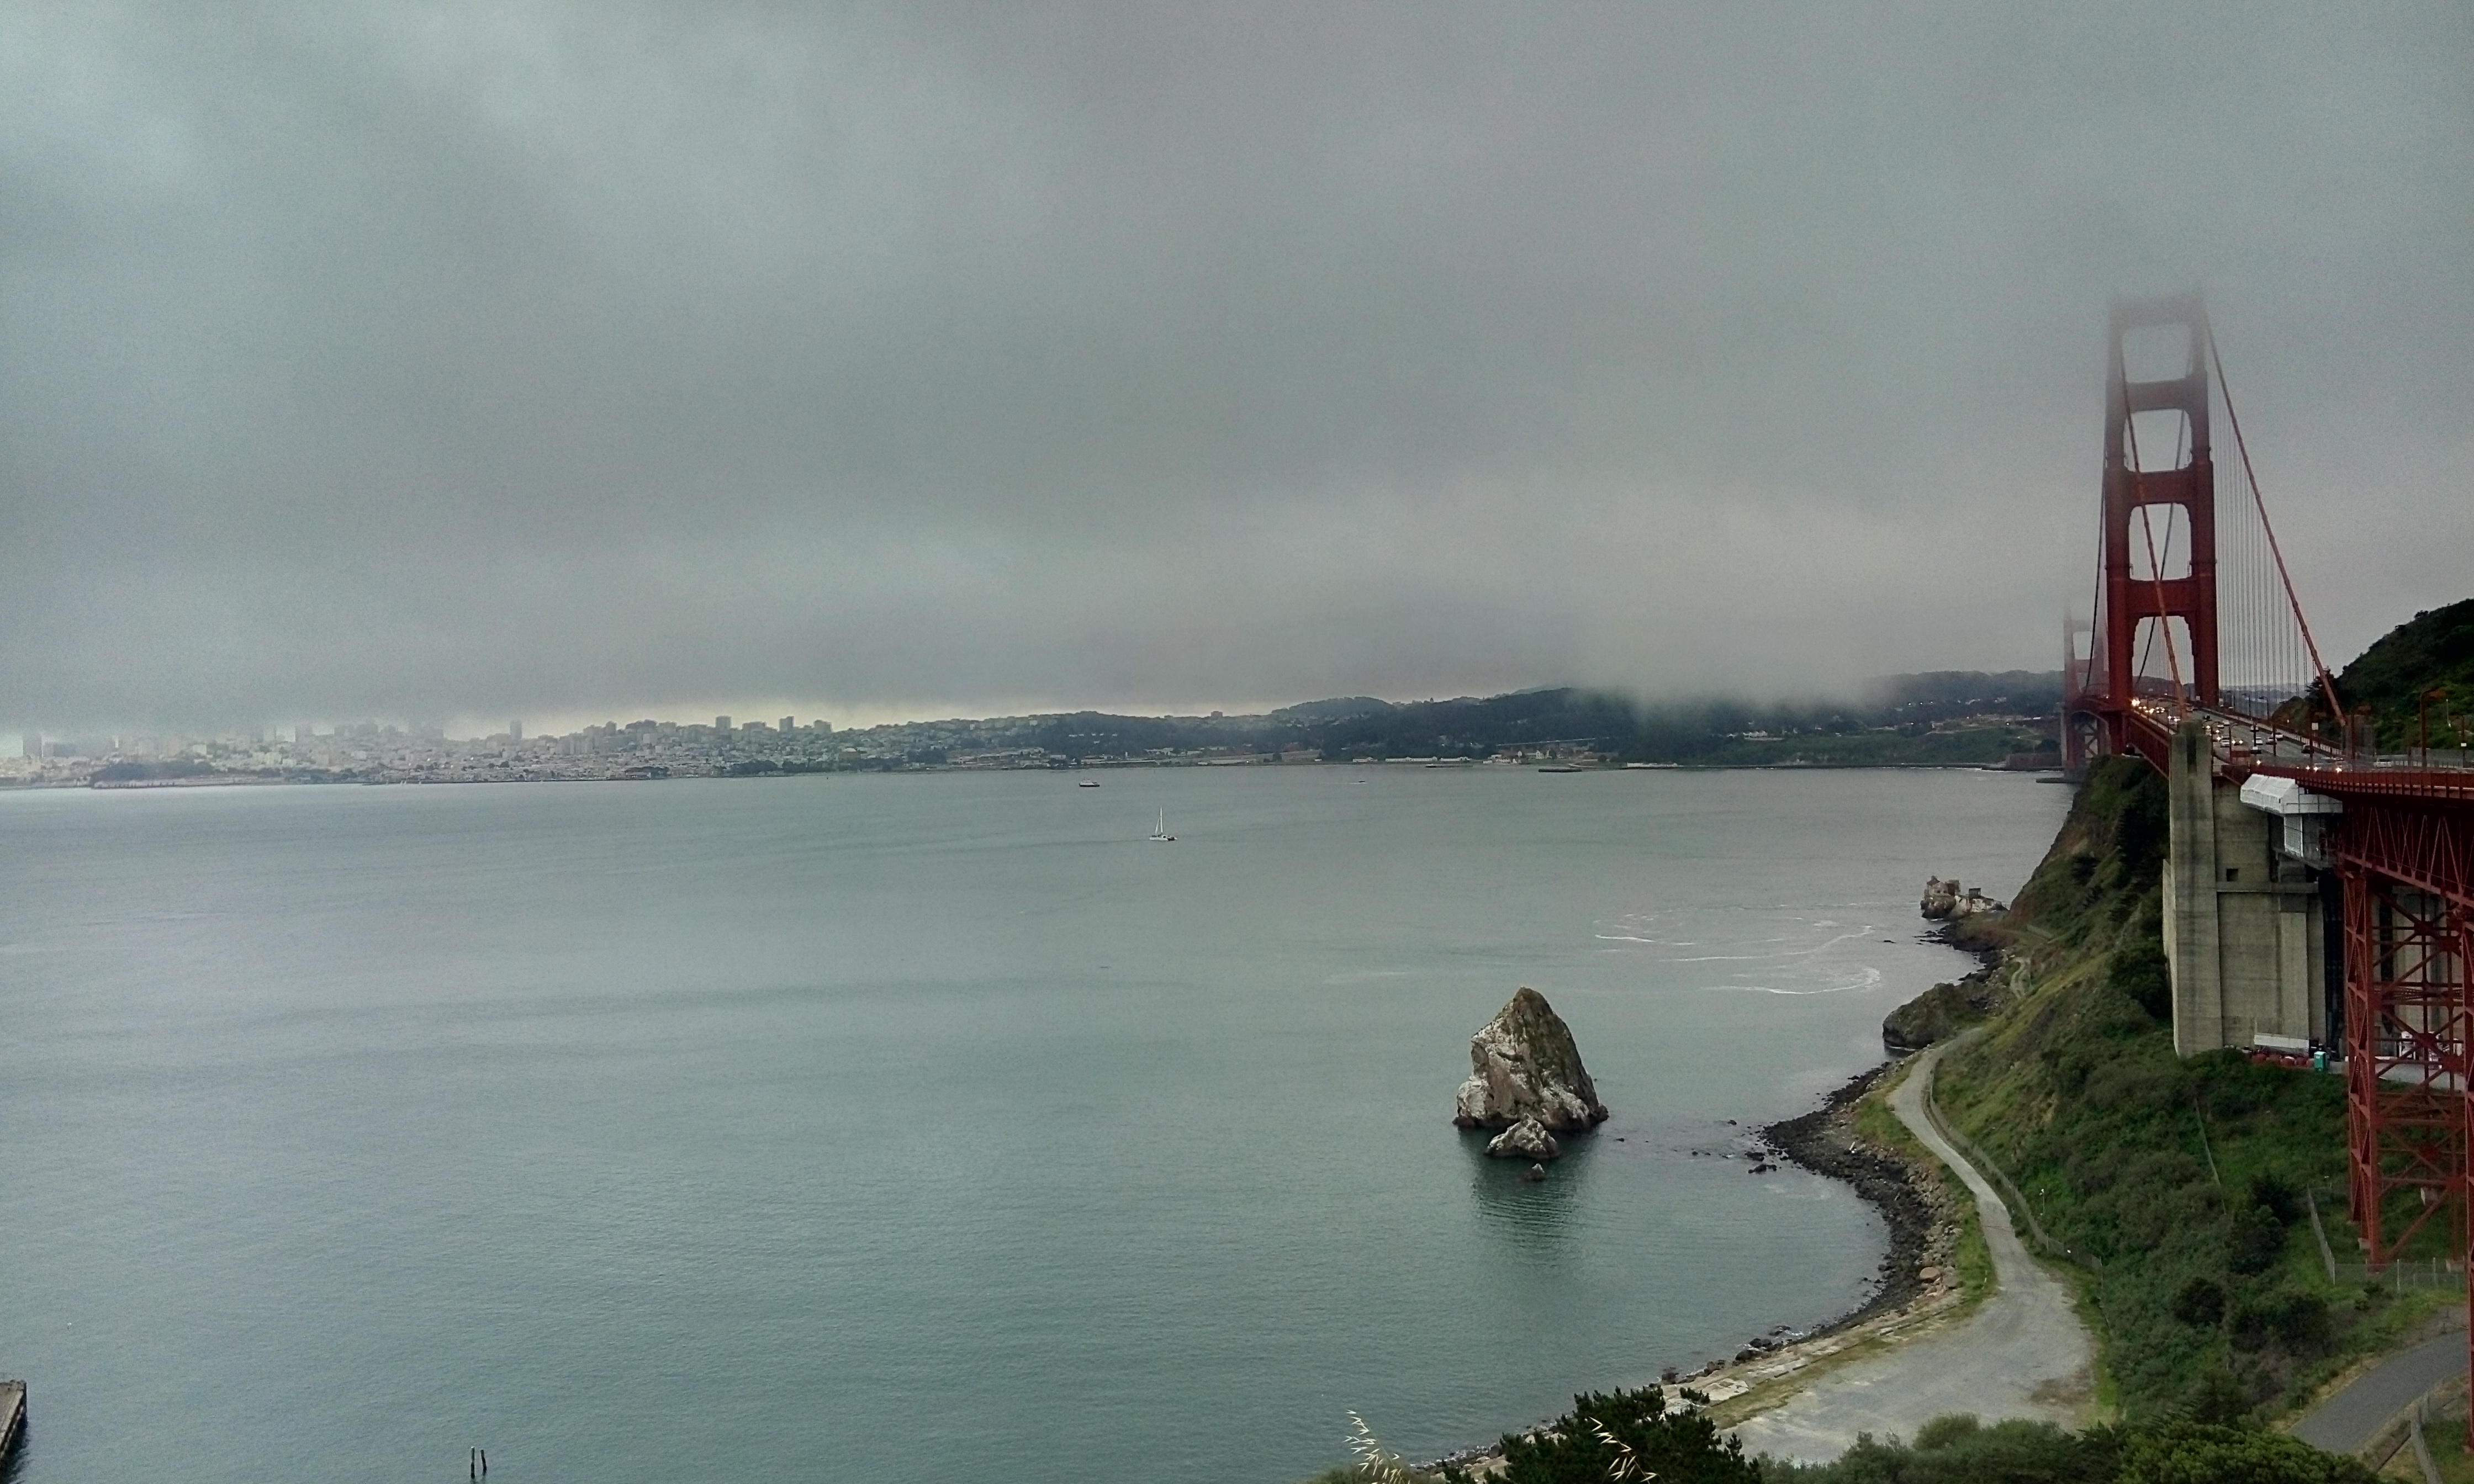
\includegraphics[width=\paperwidth,height=.5\paperheight]{21/image20160420_193101911.jpg};%
%};
\end{tikzpicture}
\newpage


Bis etwa hierhin war die Landschaft hügelig und nach einigen weiteren Meilen wurde die Küste richtig steil.
Die Straße schlängelte sich ab da so durch und die erlaubten 55~mph schafft man mit keinem Sportfahrwerk.
Zwischen 20 und 40~mph fährt man, wenn nicht beabsichtigt gute 100~m in die Tiefe zu "fahren".\\

An einem Aussichtspunkt saßen zwei Hitchhiker, die ich eingepackt hätte.
Vorausgesetzt wir wären in ihre Richtung gefahren, wobei ich mir gut vorstellen kann, dass die zwei überall hin mitgefahren wären, denn der Aussichtspunkt liegt mitten im Nirgendwo.
Der Christian hat die zwei jedoch gleich mal als Landstreicher diffamiert und sich quer gestellt.
Die nächsten Tramper gehen aber an Bord!\\

In Monterey geht es morgen ins Aquarium\dots wie spannend.


\subsection*{Fische in Glaskästen}
Gestern wollte ich mir im Wallmart noch eben zwei Einwegrasierer mitnehmen.
So wie man sie auch in Deutschland von der Tanke kennt.
Die kleinste Packungsgröße war 12.
Für 1,88~\$.\\

Was wir an Zeit für die USS Midway zu wenig, haben wir für das Monterey Bay Aquarium zu viel vorgesehen.
Der Eintrittspreis von 40~\$ pro Person steuerte sicherlich seinen Beitrag dazu.
Es war so langweilig, wie ich es erwartet hatte,
\glqq Action\grqq \, kam nur bei der Fütterung auf und selbst die war fad.
Denn die größeren Raubtierfische haben wenig Interesse an totem Fisch, fressen eh nur alle zwei bis drei Tage oder haben schon andere \glqq Beifische\grqq \, vernascht.
Neben den Fischen gab es noch Otter, Vögel und selbstverständlich ein Restaurant mit Gift Shops.
Die ganze Einrichtung soll dem Ami näher bringen, dass er nicht aller unüberlegt in sich reinfressen soll.

Finanziert wurde der Komplex über Spendengeldern von 100.000~\$ aufwärts.
Bei einem Betrag von 100.000~\$ könne man meinen dem Spender wird ein Flügel in der Attraktion gewidmet, aber ein Großspender wie Packard (HP) mit 50 Millionen sorgt dann eher dafür, dass einem für seine sechsstellige Summe gerade mal eine Klobrille gewidmet wird.
Aber es ist nicht so, dass ich überhaupt nichts lernen konnte.
Bei Ebbe umgreift Patrick Star eine Muschel, öffnet sie gewaltsam und frisst ihren Inhalt.\\

Die Fahrt nach San Francisco auf der Route~1 führte wieder an vielen Obst Plantagen vorbei auf denen sich billige Arbeitskräfte aus dem -Osten, Polen,- Süden, Mexiko, verdingen.
Wir sind dann bei ausklingendem Arbeitsverkehr am ersten Hostel angekommen und dort wäre eine Übernachtung in einem 22er Zimmer möglich gewesen, was der Prinzessin Christian nicht taugte.
Also sind wir weitergefahren zum Hostel Marin Headlands bei Sausalitos.
Dazu überquerten wir die Golden Gate Bridge, was 7.25~\$ pro Überfahrt kostet.
Abgerechnet wird das übers Kennzeichen.
Mal schauen, ob da noch was kommt.
Statt Großstadtdschungel hatten wir für die Nacht dann Natur pur.


\subsection*{Alcatraz}
Die Nacht war kurz, denn wir mussten früh raus, um zeitig über die Golden Gate Bridge zu fahren zu unserem Ziel Pier 39.
Von dort laufen die Fähren nach Alcatraz aus.
Einem Betonklumpen in der Bucht von San Francisco.
Aber wenn die Amerikaner etwas können, dann ist es die Unterhaltung.
Der Audio-Guide hauchte dem Klumpen richtig Leben ein und so wurde eine empfehlenswerte Attraktion draus.

Im Anschluss suchten wir uns eine neue Unterkunft.
Die alte war zwar schön, aber leider auch schön Abseits von allem.
Im Hostel City Central wurden wir fündig.
Den restlichen Tag wollten wir mit China Town verbringen, aber da wir in die falsche Richtung gelaufen sind, wurde es eben Little Tokyo.
Ewig konnten wir nicht umher streunen, denn für den Abend war der allwöchentliche Pub Crawl angesagt.

Dort trafen wir in erster Linie andere Deutsche, Georg und Querin aus Mittenwald, einen Würzburger, der zum Thema Akkus promoviert und mir erklären konnte warum Tesla Autos mit größerer Reichweite bauen kann als die Anderen, und noch ein paar andere Gesichter.
Summa sumarum waren wir in vier verschiedenen Pubs, eine Schwulenkneipe war auch dabei, hatten einen angenehmen Abend.


%Alcatraz
%Pier 39
%Hostel City Central
%Little Tokyo
%Pub Crawl
%
%Mittenwald (Georg + Querin (Q.))
%Würzburger 

\subsection*{Geisterstunde}
Nachdem wir am Vortag statt nach \FOREIGN{China Town} nach \FOREIGN{Little Tokyo} gelaufen sind, stand heute \FOREIGN{China Town} an.
Das regnerische Wetter zwang uns jedoch am \FOREIGN{Union Square} im Einkaufshaus \FOREIGN{Macy's} Unterschlupf zu suchen.
Dort haben wir alle acht Stockwerke nach Herrenläden abgesucht und nichts gefunden.
Beim Rausgehen ist uns dann die Werbung für das männliche Pendant 5~m weiter aufgefallen.
Das hatte nur fünf Stockwerke und dennoch keine bezahlbaren Unterhosen (36~\$ für 4).
Die Frage waschen oder kaufen ließ (im Vorfeld) nur eine Antwort zu.
Aber im gut bekannten H\&M wurde ich dann fündig (13~\$ für 3).

Die Regenwolken waren weg und wir gingen weiter.
Um uns herum wurde kein Englisch mehr gesprochen, die Passanten wurden kleiner, hatten andere Augen und waren i.d.R. gelb.
Dort habe ich dann das günstigste und \textbf{beste} Essen gefunden.
\FOREIGN{Fingerfood} versteht sich.

Am Abend speisten wir noch in der \FOREIGN{Cheesecake Factory} ehe wir an einer nächtlichen Führung durch \TOWN{San Francisco} teilnahmen.

\subsection*{Goggle}
Angedacht war \TOWN{San Francisco} mit dem Fahrrad zu erkunden, aber da wir gefühlt in den vorangegangenen Tagen schon alles gesehen hatten, checkten wir zeitig aus und fuhren weiter zur \glqq Farm\grqq\footnote{Stanford University}.
Eine der ältesten Unis in den USA, die dieses Jahr ihr 125. Bestehen feiert.
War jetzt nicht so besonders, Räume mit Gerätschaften gibt es auch an deutschen Unis.
Da sich die \FOREIGN{Stanford University} inmitten des \FOREIGN{Silicon Valley befindet, haben wir noch das ein oder andere IT Unternehmen besucht.
Bei Google war am Wochenende auch nichts los, interessant fand ich nur, dass in die Fläche und nicht in die Höhe gebaut wurde.
Durch Zufall sind wir noch auf einen Deutschen gestoßen, dessen Reisepartner nach vier Monaten Heimweh bekam und der nun die restlichen sechs Wochen alleine herum tourt.

Von \TOWN{Palo Alto} ging es weiter Richtung Yosemite National Park.
Der Weg dahin führte wieder an Plantagen vorbei, im Diner Hula frühstückten wir gegen 16~Uhr (\FOREIGN{Bowl of Oatmeal}\footnote{Haferflocken} und \FOREIGN{Pancakes}) und danach wurde die Landschaft ansehnlicher.
Erst hügeliger, dann richtig bergig.
Die \glqq Passstraße\grqq \, war wahnsinnig schön!

Im Hostel \TOWN{Groveland} genehmigten wir uns zu zweit ein achter Zimmer (45~\$ statt 35~\$).
Der Weg zu den Betten führte durch die Küche und in dieser werkelte ein französisches Paar mit dem Resultat, dass die ganze Hütte nach ihrem Essen roch.
Unser Zimmer roch auch noch am nächsten morgen, da hatte sich das Waschen der Wäsche am Abend ja gelohnt.
Am Abend besuchten wir noch die älteste Kneipe Kaliforniens den ``\FOREIGN{Iron Door Saloon}''.
Dort gab es was zu Essen, Livemusik und zu unserem Glück ein Paar, dass voll wie die Haubitzen war und Platz für uns machte.
Zu Essen gab es Burger, zu Trinken ein Dunkel das schmeckte!

Im Verlauf des Abends erzählte mir die \glqq Anführerin\grqq \, der \FOREIGN{Bachelorparty}\footnote{Junggesellenabschied}, dass der Yosemite doch so schön ist.
Man erkenne das Wirken Gottes.
Naja, mal sehen.

Zum Schluss wurden wir dann noch Zeuge einer Handgreiflichkeit, die ein Einheimischer wie folgt kommentierte.

\begin{quote}
	\FOREIGN{That's how we treat our girls. We pull them by their hair.}
\end{quote}


\subsection*{Half-dome}
Einmal im Jahr gibt es eine Woche in der alle Nationalparks keinen Eintritt kosten.
Dafür wird nach einer Spende (Donation) gefragt.
Wir haben den letzten Tag dieser erwischt, entsprechend belebt war es.
Aber sicherlich nicht so belebt, wie in der Hochsaison.

Vom Yosemite National Park Schild bis zum Passierhäuschen waren es wieder gute 30~Meilen.
Auf dem Weg dahin hielten wir an einem Aussichtspunkt an, von dem man das Resultat eines Waldbrandes betrachten konnte.
Dort gab es eine Haltevorrichtung zum Fotografieren und die Bitte das Foto auf einer social media Plattform mit dem Hashtag #rimfire01 zu posten.
Cleveres Outsourcen!

Wir sind ins Valley gefahren, um von dort den Upper Falls Trail in Angriff zu nehmen.
Ich bin mit Winterjacke los und nach ein paar Höhenmeter in der Sonne habe ich mich darüber geärgert die Jacke überhaupt mitgenommen zu haben.
Der Trail war mit 5 bis 7 Stunden angegeben, nach rund 2~Stunden waren wir bereits oben.
Dann schlug aber das Wetter um und ich war total glücklich meine Jacke mitgenommen zu haben.
Vollkommen durchnässt kamen wir dann am Auto an und fuhren nach Mariposa unserer Unterkunft.

Dort gingen wir mal etwas gehobener Essen und siehe da, beim 24~\$ Beef Steak war eine Vorspeise mit dabei und die Crème Brulée stellten sie uns auch nicht in Rechnung.
Insgesamt war das Abendessen nicht wesentlich teurer als sonst, dafür geschmacklich 1a.


\subsection*{Sequoias}
Die Nacht haben wir Dank vierfach Schloss unverletzt überlebt und weil seit gestern das Auto meint wir sollten das Öl wechseln, haben wir den Ölstand kontrolliert.
Der hat gepasst und der Kundensupport meinte wir sollen uns nichts dabei denken und weiter fahren.
So haben wir das dann auch gemacht.

Gegen 10~Uhr waren wir wieder auf den Weg in den Yosemite National Park mit \FOREIGN{Mariposa Grove} als Ziel.
Dort gab es Sequoia Bäume.
In etwa ein halbes Dutzend.
Die sind zum einen riesig, zum anderen feuerfest!
Sie brauchen die Waldbrände sogar, damit das Feuer die schneller wachsende Konkurrenz zu Dünger umwandelt und weil sich die Zapfen mit den Samen nur bei einem Brand öffnen.

Anschließend sind wir wieder über Mariposa aus dem Park gefahren, da die Parkranger die andere Route vor unserer Nase dicht gemacht hatten.
War sicherlich gesünder für uns, denn schneetauglich schien unsere Karre nicht zu sein.

Die Landschaft war in erster Linie wieder von Plantagen geprägt.
Kilometerweit ein Baum neben dem anderen, schön maschinengerecht in Reih und Glied angeordnet.
Im \glqq Zentrum\grqq \, lag die Ortschaft \TOWN{Orange Cove} und jetzt ist auch schon verraten, um was für Plantagen es sich handelte.
Am Plantageneingang fand sich noch die Warnung \FOREIGN{Spring Flood Area}, was bei dem erodierten Boden überhaupt kein Wunder ist.

Ein Arbeitskollege vom Christian hatte uns noch den \FOREIGN{Bass Lake} nahe \TOWN{Oakhurst} empfohlen.
Die Gegend war ja ganz nett, aber anscheinend waren wir auf der falschen, der zugebauten Uferseite.

Kurz vor \TOWN{Three Rivers} kamen wir noch an einem weiteren See vorbei, dem \FOREIGN{Lake Kaweah}.
Das war bist jetzt die erste Anlage, die

\begin{tikzpicture}[remember picture, overlay]
\node[inner sep=0pt, yshift=-.25\paperheight] at (current page.north) {%
	\includegraphics[angle=0,width=\paperwidth,height=.5\paperheight]{25/image20160425_182848870.jpg};%
};
\end{tikzpicture}

\vspace*{.35\paperheight}
\noindent
die Besuchergebühren hatte.
War aber keiner da.

In Oakhurst hatten wir gegen 14~Uhr unser Frühstück nachgeholt und da das auch noch bis in den späten Abend anhielt, substituierten wir das Abendessen durch Bier.


\subsection*{Noch mehr Sequoias}
Während in Mariposa vier Schlösser für unsere Unversehrtheit sorgten, übernahm dies in \TOWN{Three Lakes} ein indisches Gebet.
Es gab mal wieder ein Frühstück, das aus Toast, Kuchen, Cornflakes und Waffeln bestand.
Besteck war aus Plastik, ebenso die Teller und am Schluss landete alles im Müll.
Man aß quasi Müll von Müll mit Müll.

Im Yosemite National Park gab es einzelne Flecken an denen Sequoias wachsen, aber es gibt auch einen eigenen Sequoia National Park.
Der war unser heutiges Vormittagsprogramm.
Und dort ist es dann passiert!
Dem Christian waren die Jungs auf den ersten Blick wieder nicht koscher genug, aber ich saß am Steuer und so hielten wir an.
Räumten die Rücksitzbank auf und die Herren waren an Bord.
Neusseländer hatten wir da aufgegabelt, die mit ihrem Wohnmobil nicht bis hoch zu den Sequoias fahren konnten.
Sie waren in den USA, da sie eine Firma betreiben um mit Drohnen zu filmen.
Dafür erhielten sie einen Preis und machten danach noch Urlaub.
Am Informationszentrum trennten sich die Wege wieder, wir lasen uns schlau und wer hätte es gedacht, die Amis räumen doch glatt ein, dass sie in der Vergangenheit ganz falsch mit den Sequoias umgegangen sind.
Unter anderem gab es an Ort und Stelle mal eine Tankstelle und durch das Löschen von Waldbränden kamen auch keine neuen Sequoias hinzu.

Nachdem wir genug große Bäume gesehen hatten, fuhren wir weiter zum \TOWN{Death Valley}.
500~km dürften es locker gewesen sein.
Da unser Bett für die Nacht jedoch auf der anderen Seite lag, fuhren wir gleich mal durch.
Ein gewisser Nervenkitzel war dabei, der Tankinhalt war recht überschaubar und im \TOWN{Death Valley} gibt es nur eine einzige Tankstelle mit entsprechenden Preisen.

Angekommen sind wir in \TOWN{Beatty} und die dortige Tankstelle hatte auch wieder bessere Preise.
Da wir im Ort Pizzen zum Mitnehmen bestellen wollten, hatten wir keine Pässe mitgenommen, was zum ersten Mal überhaupt kein Problem darstellte.
So konnten wir die Wartezeit von 30~Minuten mit einem guten Hellen überbrücken.

\newpage
\thispagestyle{empty}
\begin{tikzpicture}[remember picture, overlay]
\node[inner sep=0pt] at (current page.center) {%
	\includegraphics[angle=0,width=\paperwidth,height=\paperheight]{26/image20160426_101234649.jpg};%
};
\end{tikzpicture}
\newpage





\subsection*{Death Valley}
Nach der gestrigen Durchfahrt, wollten wir uns heute das \glqq Tal des Todes\grqq\, genauer ansehen.
Wir machten halt bei den Dünen, liefen die nächste und höchste hoch und mit fast verbrannten Füßen wieder runter.
Ein Hinweisschild wies einen darauf hin die Dünen nur am Morgen oder am Abend zu begehen.
Macht absolut Sinn.

Als nächstes hielten wir bei einer ehemaligen Abbaustätte, die sich nicht lange lohnte.
Dann gab es noch ein obligatorisches Besucherzentrum und von dort fuhren wir erst einen Salzsee und tiefsten Punkt \FOREIGN{Bad Water Basin} und anschließend \FOREIGN{Dante's View} an.
Bei \FOREIGN{Dante's View} blickt man auf den Salzsee, nur eben von einer erhöhten Position.

\thispagestyle{empty}
\begin{tikzpicture}[remember picture, overlay]
\node[inner sep=0pt, yshift=.25\paperheight] at (current page.south) {%
	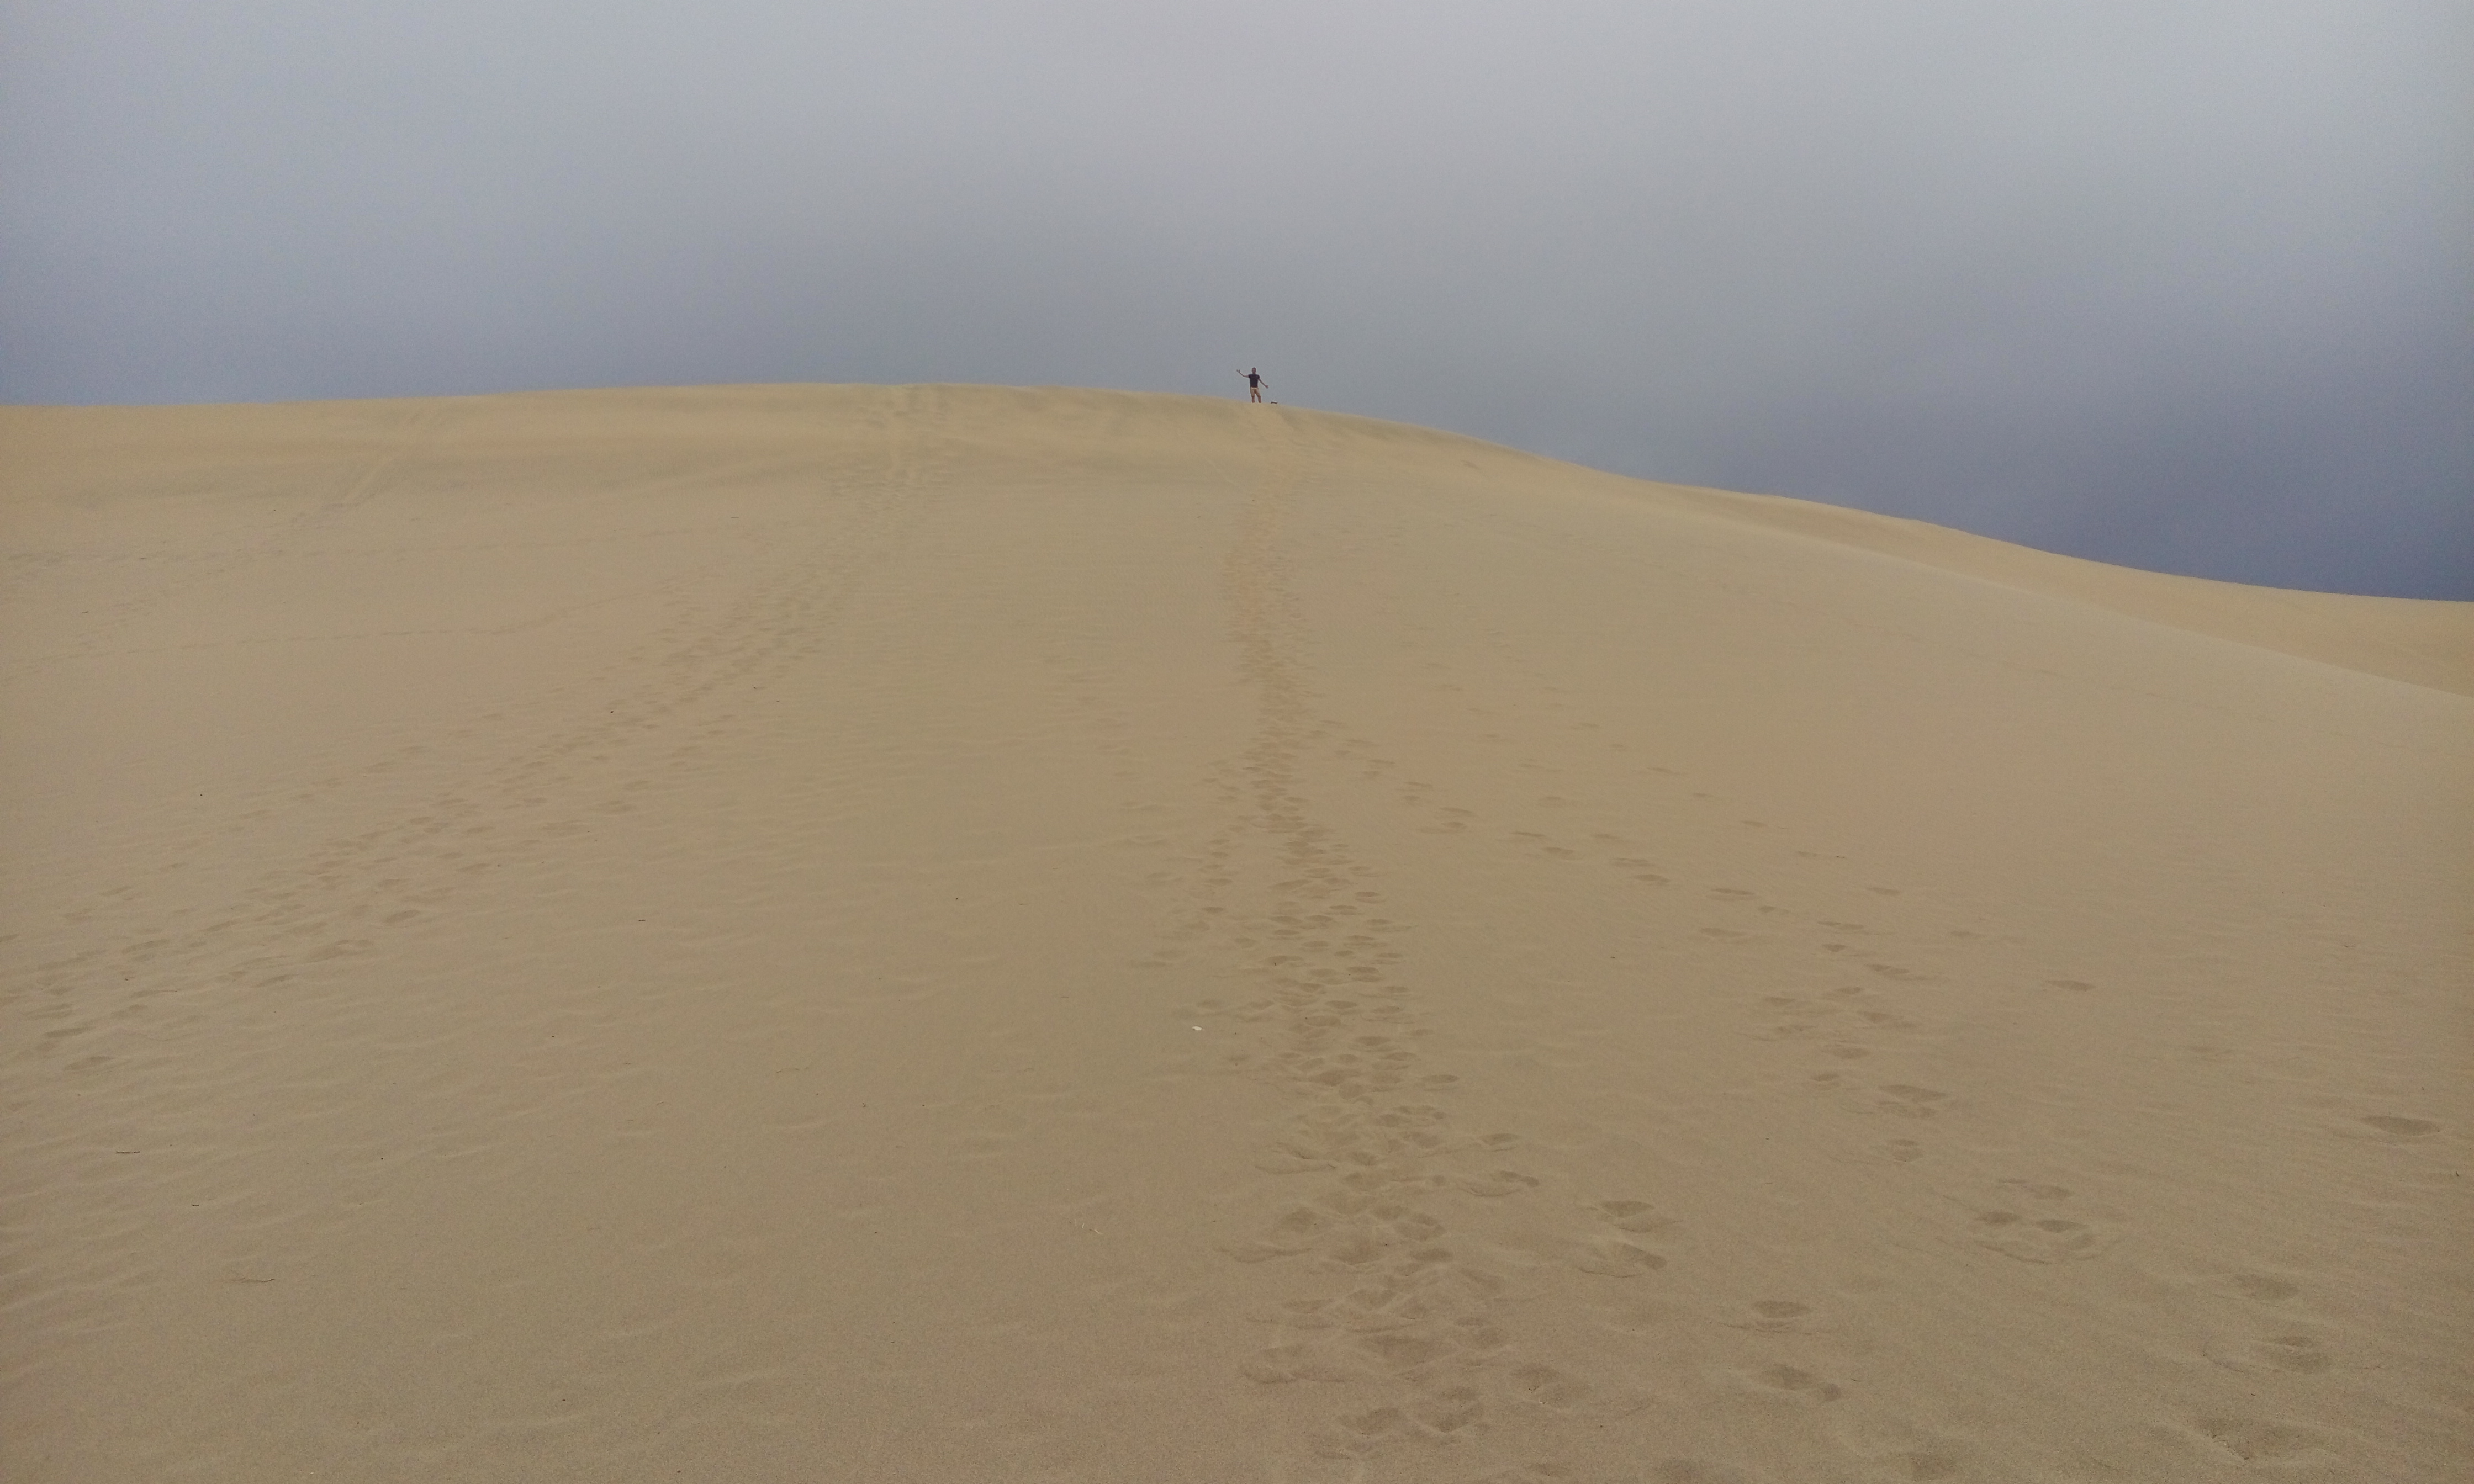
\includegraphics[angle=0,width=\paperwidth,height=.5\paperheight]{27/image20160427_111303992.jpg};%
};
\end{tikzpicture}
\newpage

\thispagestyle{empty}
\begin{tikzpicture}[remember picture, overlay]
\node[inner sep=0pt, yshift=-.25\paperheight] at (current page.north) {%
	\includegraphics[angle=0,width=\paperwidth,height=.5\paperheight]{27/image20160427_131909168.jpg}%
};
\node[inner sep=0pt, yshift=.25\paperheight] at (current page.south) {%
	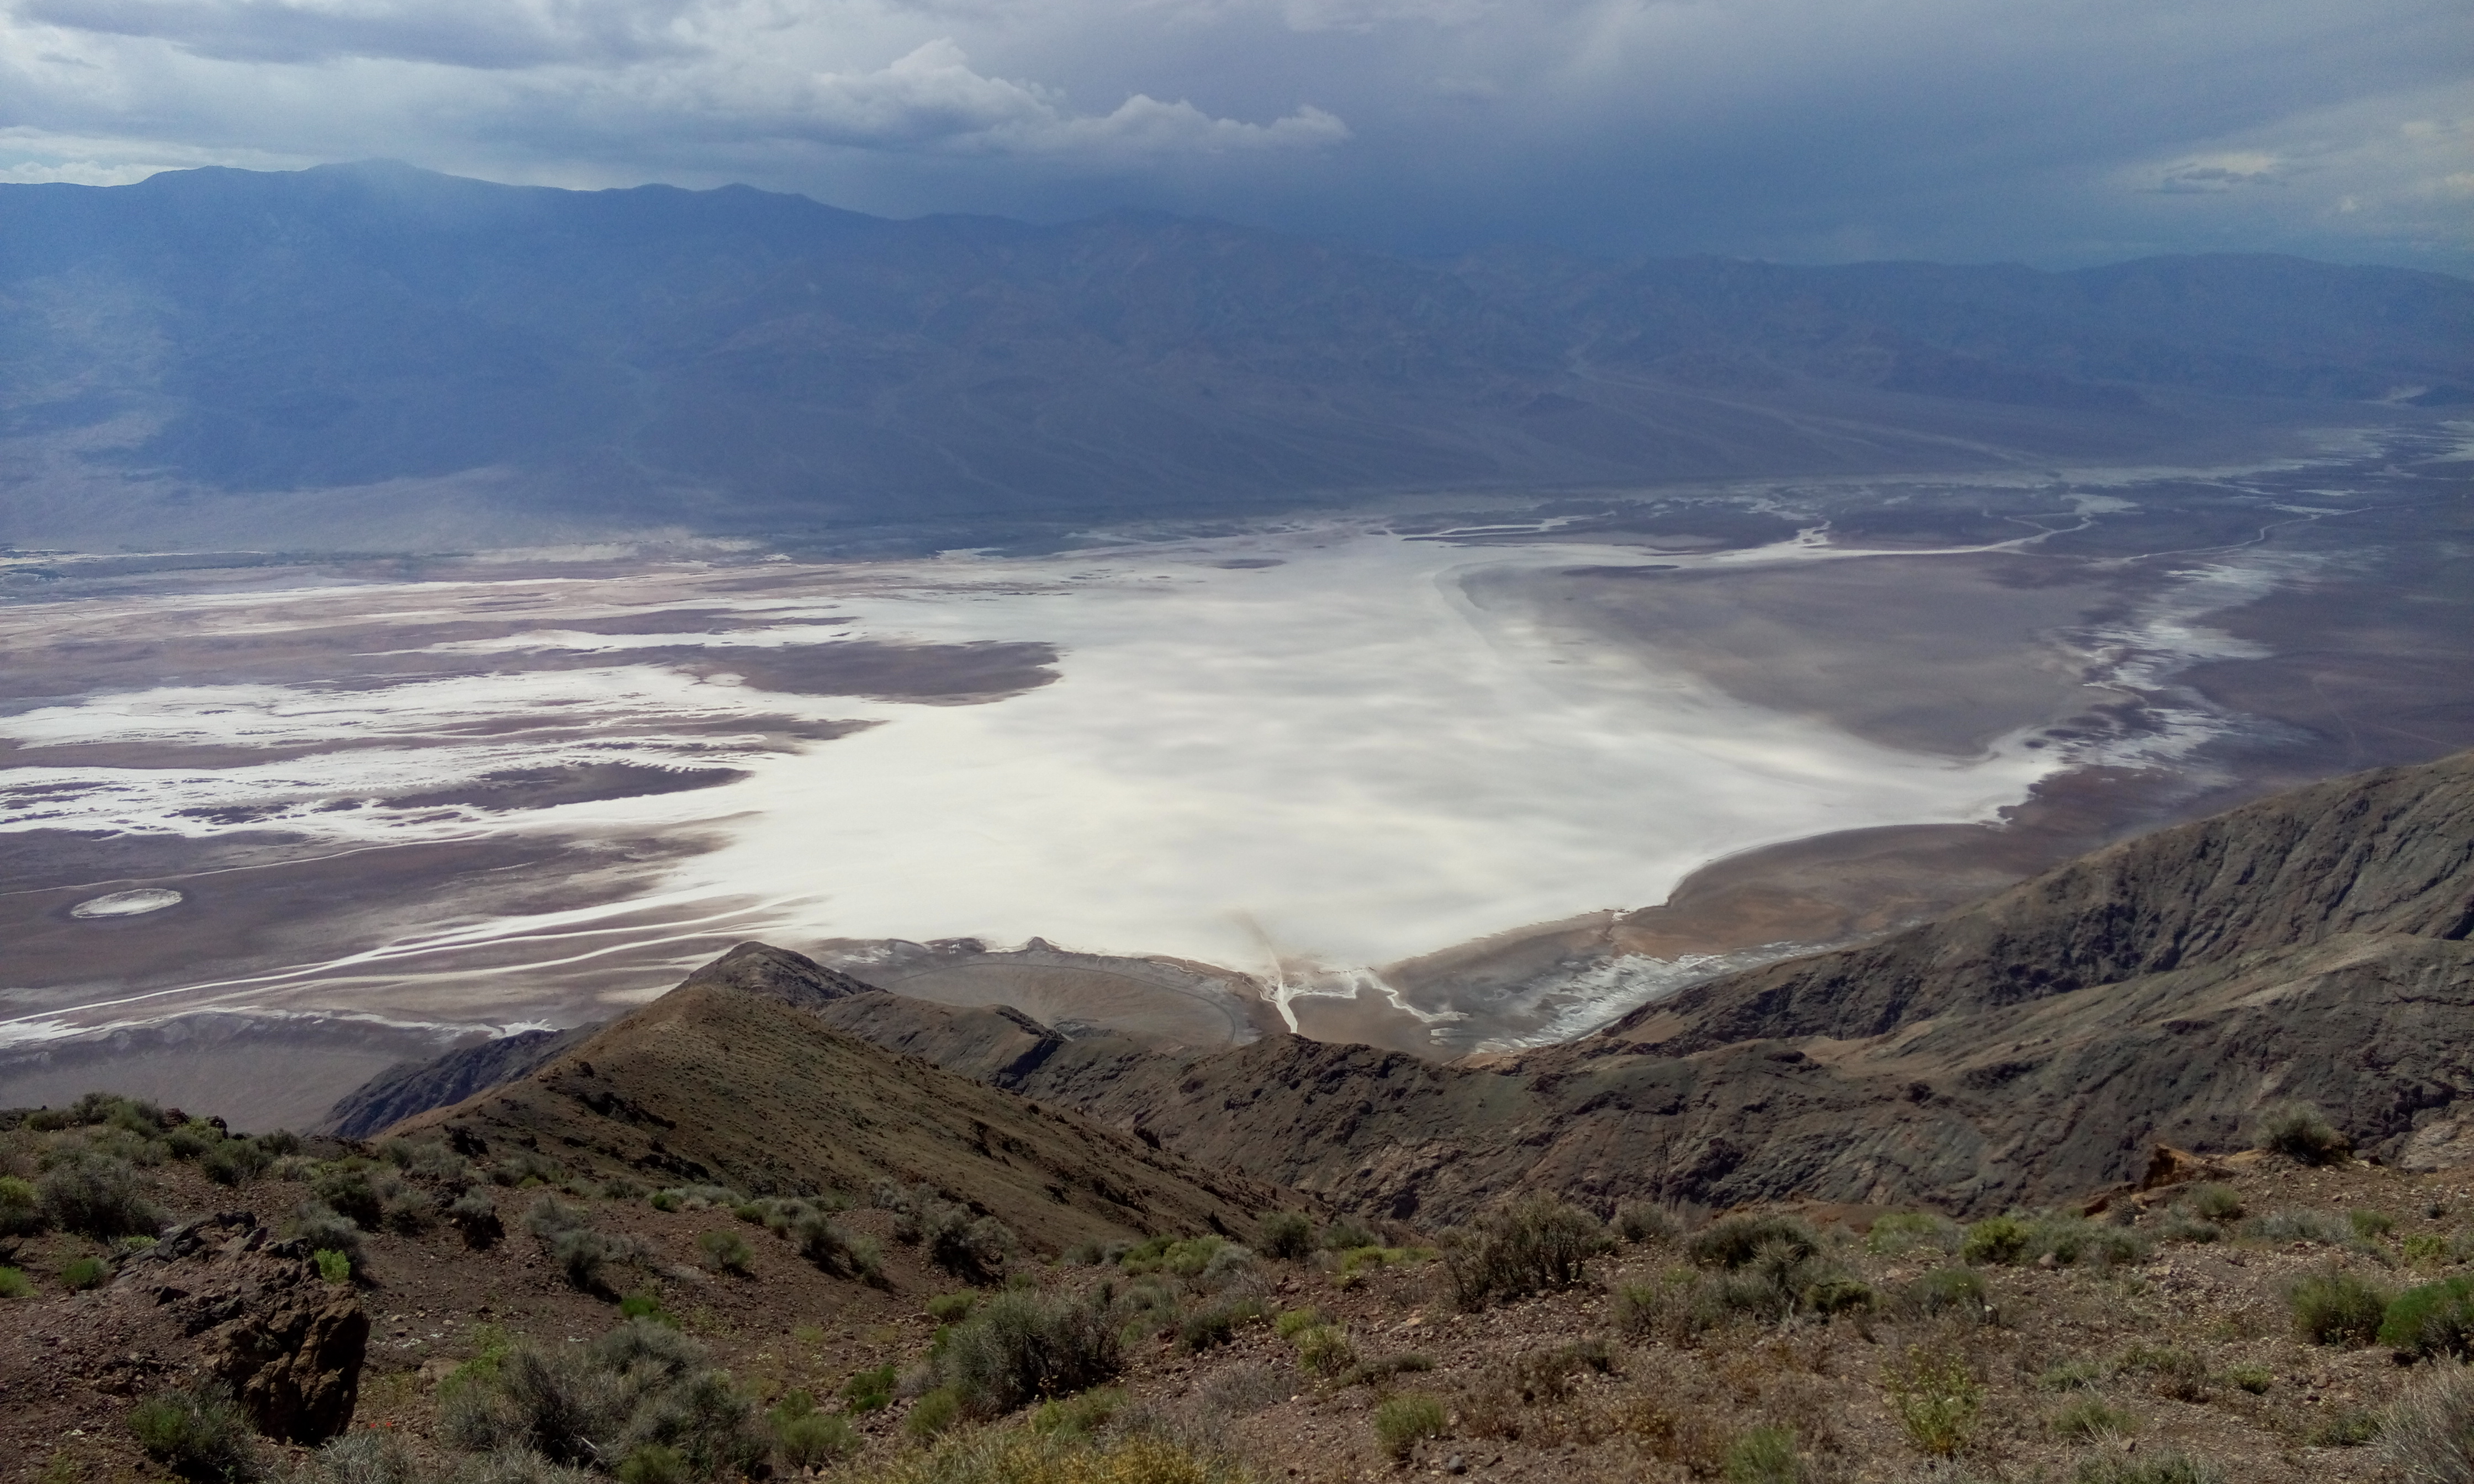
\includegraphics[angle=0,width=\paperwidth,height=.5\paperheight]{27/image20160427_144208822.jpg}%
};
\end{tikzpicture}
\newpage

Als Nachtlager stand wieder Las Vegas an und so machten wir uns auf den Weg.
Statt auf die Schatzinsel verschlug es uns zum Zirkus.
Im \FOREIGN{Circus Circus} war zum einen die Nacht spott billig, zum anderen hat das Hotel einen eigenen Freizeitpark mit Achterbahnen!

Am Abend sind wir nochmal um die Häuser gezogen und haben mal wieder Ausländer angetroffen.
Dieses Mal Österreicher.
Die hatten am Vortag erfolgreich 10~\$ am Roulettetisch auf eine Zahl gesetzt und bestellten nun unbeschwerter.


\subsection*{El Loco + Canyon Blaster}
Der Urlaub neigt sich so langsam dem Ende, was mir ganz recht ist, denn seit ein paar Tagen ist meine Kreditkarte gesperrt.
Daheim erfahre ich dann von meiner Bank, dass ich
\begin{quote}
	am 27.04.2016 um 16:59:05 bei Rajeshwari Electricals in \TOWN{Bangalore}, also Indien, 
\end{quote}
Elektrokram gekauft haben will.
Ohne den Christian wäre ich jetzt ziemlich aufgeschmissen.
Wie kann man auch nur mit einer Kreditkarte los ziehen\dots

Zum Einkaufen sind wir drei Meilen zur Mall gelaufen und wieder zurück.
Dann war es auch schon halb fünf und wir mussten ja noch in den \FOREIGN{Circus Circus} Freizeitpark.
Die zwei Achterbahnen \FOREIGN{El Loco} und der \FOREIGN{Canyon Blaster} lachten uns an.
Da der \FOREIGN{El Loco} als so \glqq brutal\grqq \, beworben wurde, setzten wir uns erstmal in den \FOREIGN{Canyon Blaster}.
Mit zwei Loopings, Schrauben und steilerem Gefälle war der aber deutlich brutaler als der luschige \FOREIGN{El Loco}.

Anschließend sind wir noch bei leichtem Nieselregen in den hoteleigenen \FOREIGN{Whirl Pool} und wurden prompt von der \FOREIGN{Security} darauf hingewiesen, das der Pool geschlossen ist.

Am Abend regnete es dann richtig und so mussten wir im Hotel auf Nahrungssuche gehen.
Das Steakhouse klang erstmal interessant, verjagte uns aber mit seinen Abwehrangeboten.
40~\$ für Vorspeisen\dots
So gingen wir zum Buffet und aßen natürlich viel zu viel.

Anschließend waren wir noch in der hoteleigenen Karaoke-Bar in der um 22$^{30}$~Uhr noch ein Kindergeburtstag gefeiert wurde.
Die zwei Kinder waren von dem Ganzen nicht so begeistert wie ihre Erziehungsberechtigten.
Undankbare Bratzen.


\subsection*{Heimwärts}
Rückfahrt nach \TOWN{Salt Lake City}, \FOREIGN{BeerHive}

\subsection*{Rückflug}
Der letzte Tag bestand im Wesentlichen darin zu packen und unseren Müll zu entsorgen.
Nach fast drei Wochen \FOREIGN{Roadtrip} hatte sich einiges im Auto angesammelt.
Das wichtigste Utensil, die Kühlbox, verblieb im Hotelzimmer.
Vielleicht konnte ja das \FOREIGN{Housekeeping} etwas damit anfangen\dots

Am Salt Lake City International Airport können sehr oft Familien beobachtet werden, die ihre Kinder mit Plakaten verabschieden oder begrüßen.
Denn von jedem \glqq richtigen\grqq\, Mormonen wird erwartet auf eine zweijährige Mission zu gehen.

Über \TOWN{Amsterdam} ging es wieder nach Hause.



\subsection*{Zahlen}
Zu guter Letzt sei noch festgehalten was uns der Spaß in etwa gekostet hat.
Die Zahlen sind also mehr oder weniger noch \textcolor{white}{durch}

\thispagestyle{empty}
\begin{tikzpicture}[remember picture, overlay]
\node[inner sep=0pt, yshift=.25\paperheight] at (current page.south) {%
	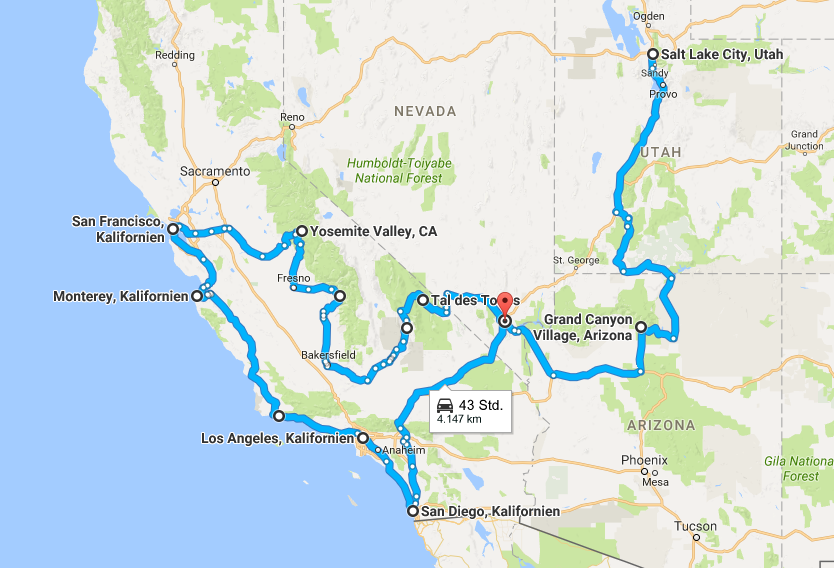
\includegraphics[angle=0,width=\paperwidth,height=.5\paperheight]{route_kleiner.png};%
};
\end{tikzpicture}
\newpage

\noindent
durch zwei zu teilen.
Wobei eine Übernachtung für eine Person nicht sonderlich günstiger ist als eine Übernachtung für zwei.

In den drei Wochen haben wir insgesamt 4646,43~€ durchgebracht. Dabei entfallen 1741,66~\$ auf die Übernachtungen, 1470,50~\$ auf Essen und Getränke und im Rest steckt der Benzin, der Mietwagen, die Einkäufe und die Tickets für die Attraktionen und National Parks.



%\cleardoublepage{}
%\newpage
%\thispagestyle{empty}
%\begin{tikzpicture}[remember picture, overlay]
% \node[inner sep=0pt] at (current page.center) {%
%  \includegraphics[width=\paperwidth,height=\paperheight]{images/EuropakarteStrecke.png};%
%};
%  \node[black,fill=white,text width=10em] (blub) at (0.5,0) {Distanz etwa 3.600~km}; %
%\end{tikzpicture}


%%%%%%%%%%%%%%%%%%%%%%%%%%%%%%%%%%%%%%%%%%%%%%%%%%%%%%%%%%%%%%%%%%%%%%%%%%%%%%%%


%\bibliographystyle{plain}
%\bibliography{bibliography}
%\begin{theindex}
%\printindex


\end{document}
